\documentclass[11pt]{article}

\usepackage{amsmath, amssymb}
\usepackage{graphicx}
\usepackage{float}
\usepackage{geometry}
\usepackage{booktabs}
\usepackage{hyperref}
\usepackage{titlesec}
\titlespacing*{\section}{0pt}{*1.2}{*0.5}
\titlespacing*{\subsection}{0pt}{*1.0}{*0.3}

\geometry{margin=1in}

\title{\textbf{Predicting Hospital Readmission in Diabetes Patients}}
\author{Nathan Gin, Alexander Yu, Nhan Nguyen \\
CS273A Machine Learning}
\date{}

\begin{document}
\maketitle

\section{Introduction}

Unplanned hospital readmissions are costly and often indicate poor transitions from hospital care to home care.
Patients with diabetes are high risk because they tend to have multiple medical conditions, medication, and visits with the healthcare system.
Accurate prediction of readmission risk can help improve follow-up resources and improve patients lives.

The goal is to build and compare several machine learning models for predicting whether a hospitalized diabetic patient will be readmitted after discharge.
This task serves as a case study in feature design, model selection, and complexity control. 

We first perform exploratory analysis to understand missingness patterns, outcome balance, and basic relationships between demographics and the other variables. We use these insights to guide preprocessing.
Next, we explore techniques less focused on in class such as Random Forests, SVMs with RBF kernels, and Neural Networks where we tune their hyperparameters.
After, we apply stratified cross-validation for parameter selection and inspect complexity curves to examine under-fitting and over-fitting.
Finally, we evaluate all models on a separate test set and compare accuracy, precision, recall, F1, and ROC--AUC.

\section{Data and Preprocessing}

\subsection{Dataset and target definition}

The Diabetes 130--US Hospitals dataset contains 101{,}766 encounters and about 50 variables, including demographics, ICD-9 diagnosis codes, lab results, procedures, medication use, and admission/discharge information.
The original outcome variable \texttt{readmitted} has three levels: ``NO'', ``$<30$'' (readmitted within 30 days), and ``$>30$'' (readmitted at some later time).

For this project we define a binary target for readmission
\[
y =
\begin{cases}
1 & \text{if readmitted $<30$ or $>30$},\\
0 & \text{if NO readmission is recorded.}
\end{cases}
\]
Under this definition the cleaned dataset has 99{,}340 encounters with about 52.9\% non-readmitted and 47.1\% readmitted, which is substantially more balanced than the original three-class formulation.

Figure 1 shows the raw distribution of readmission categories and Figure 2 shows how age relates to readmission.

\begin{figure}[H]
\centering
\begin{minipage}{0.47\linewidth}
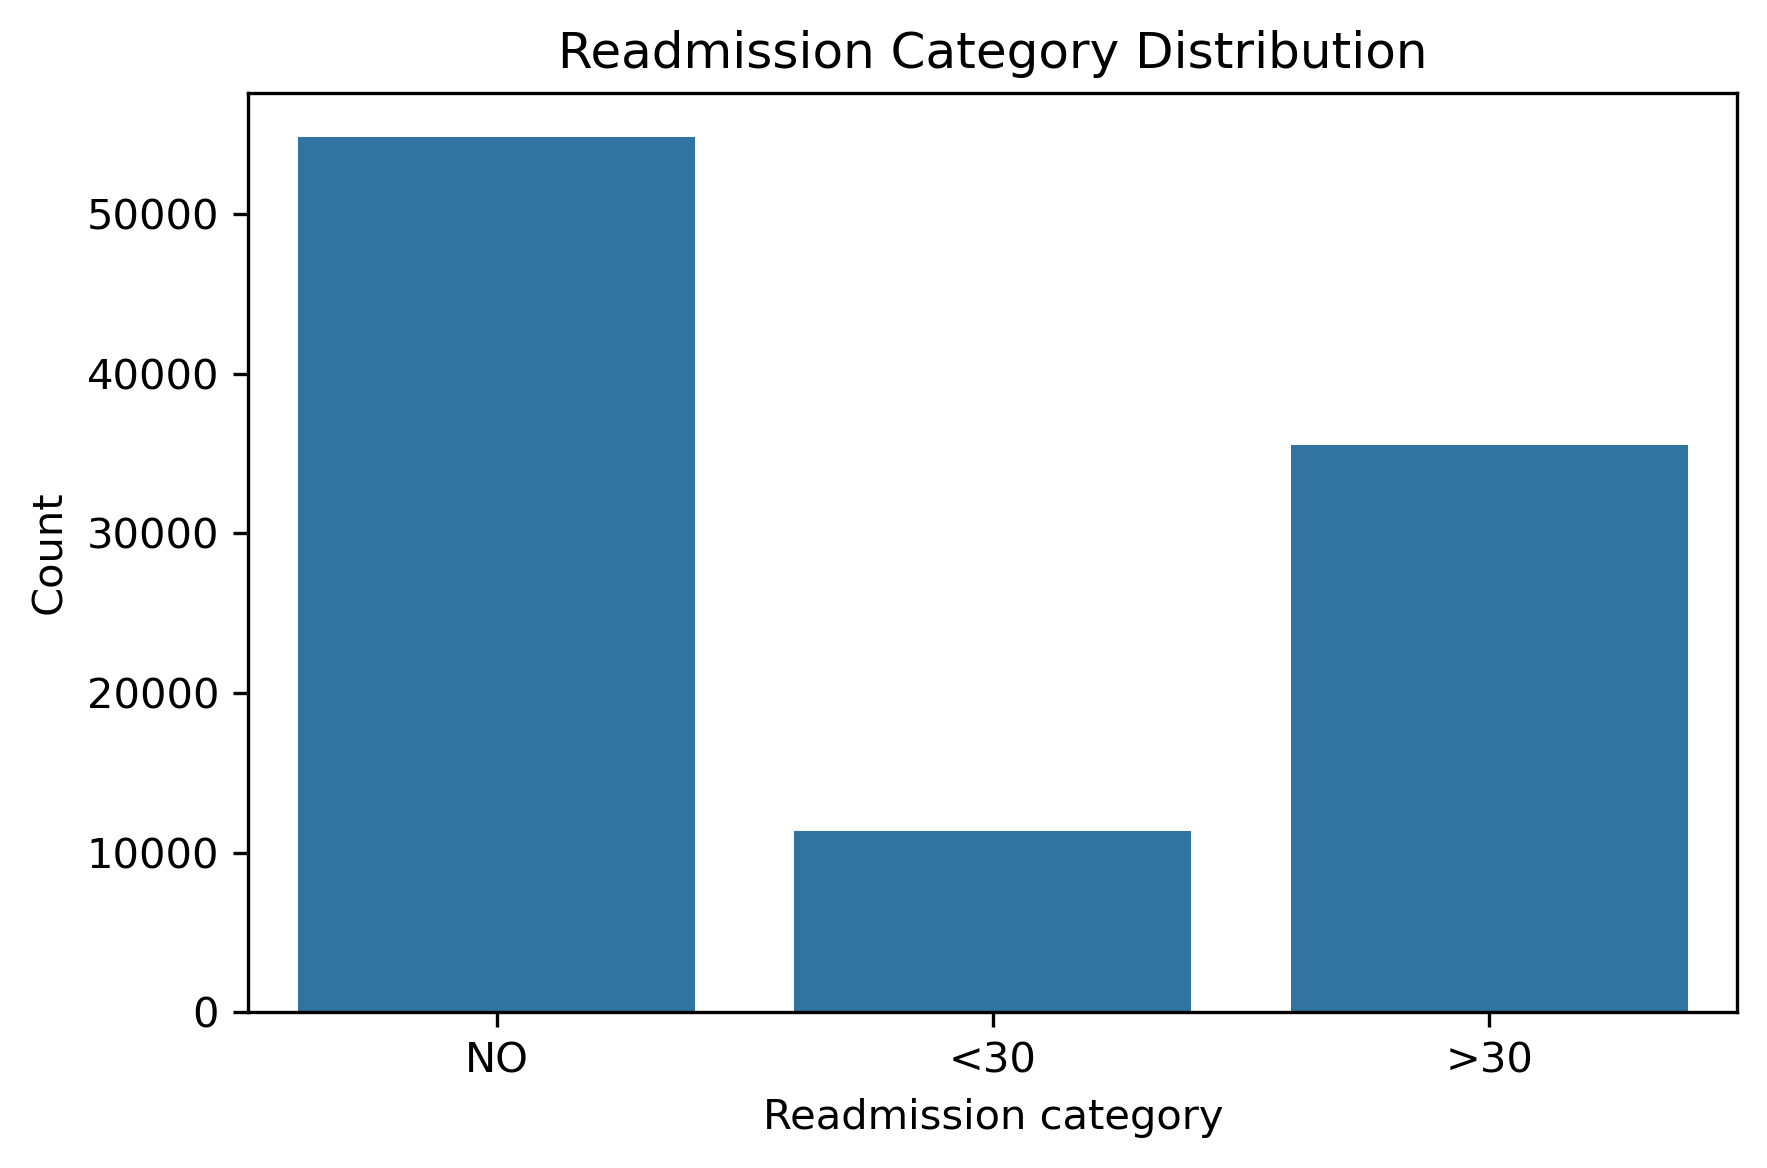
\includegraphics[width=\linewidth]{fig_readmission_distribution.png}
\caption{Raw readmission categories.}
\end{minipage}
\hfill
\begin{minipage}{0.47\linewidth}
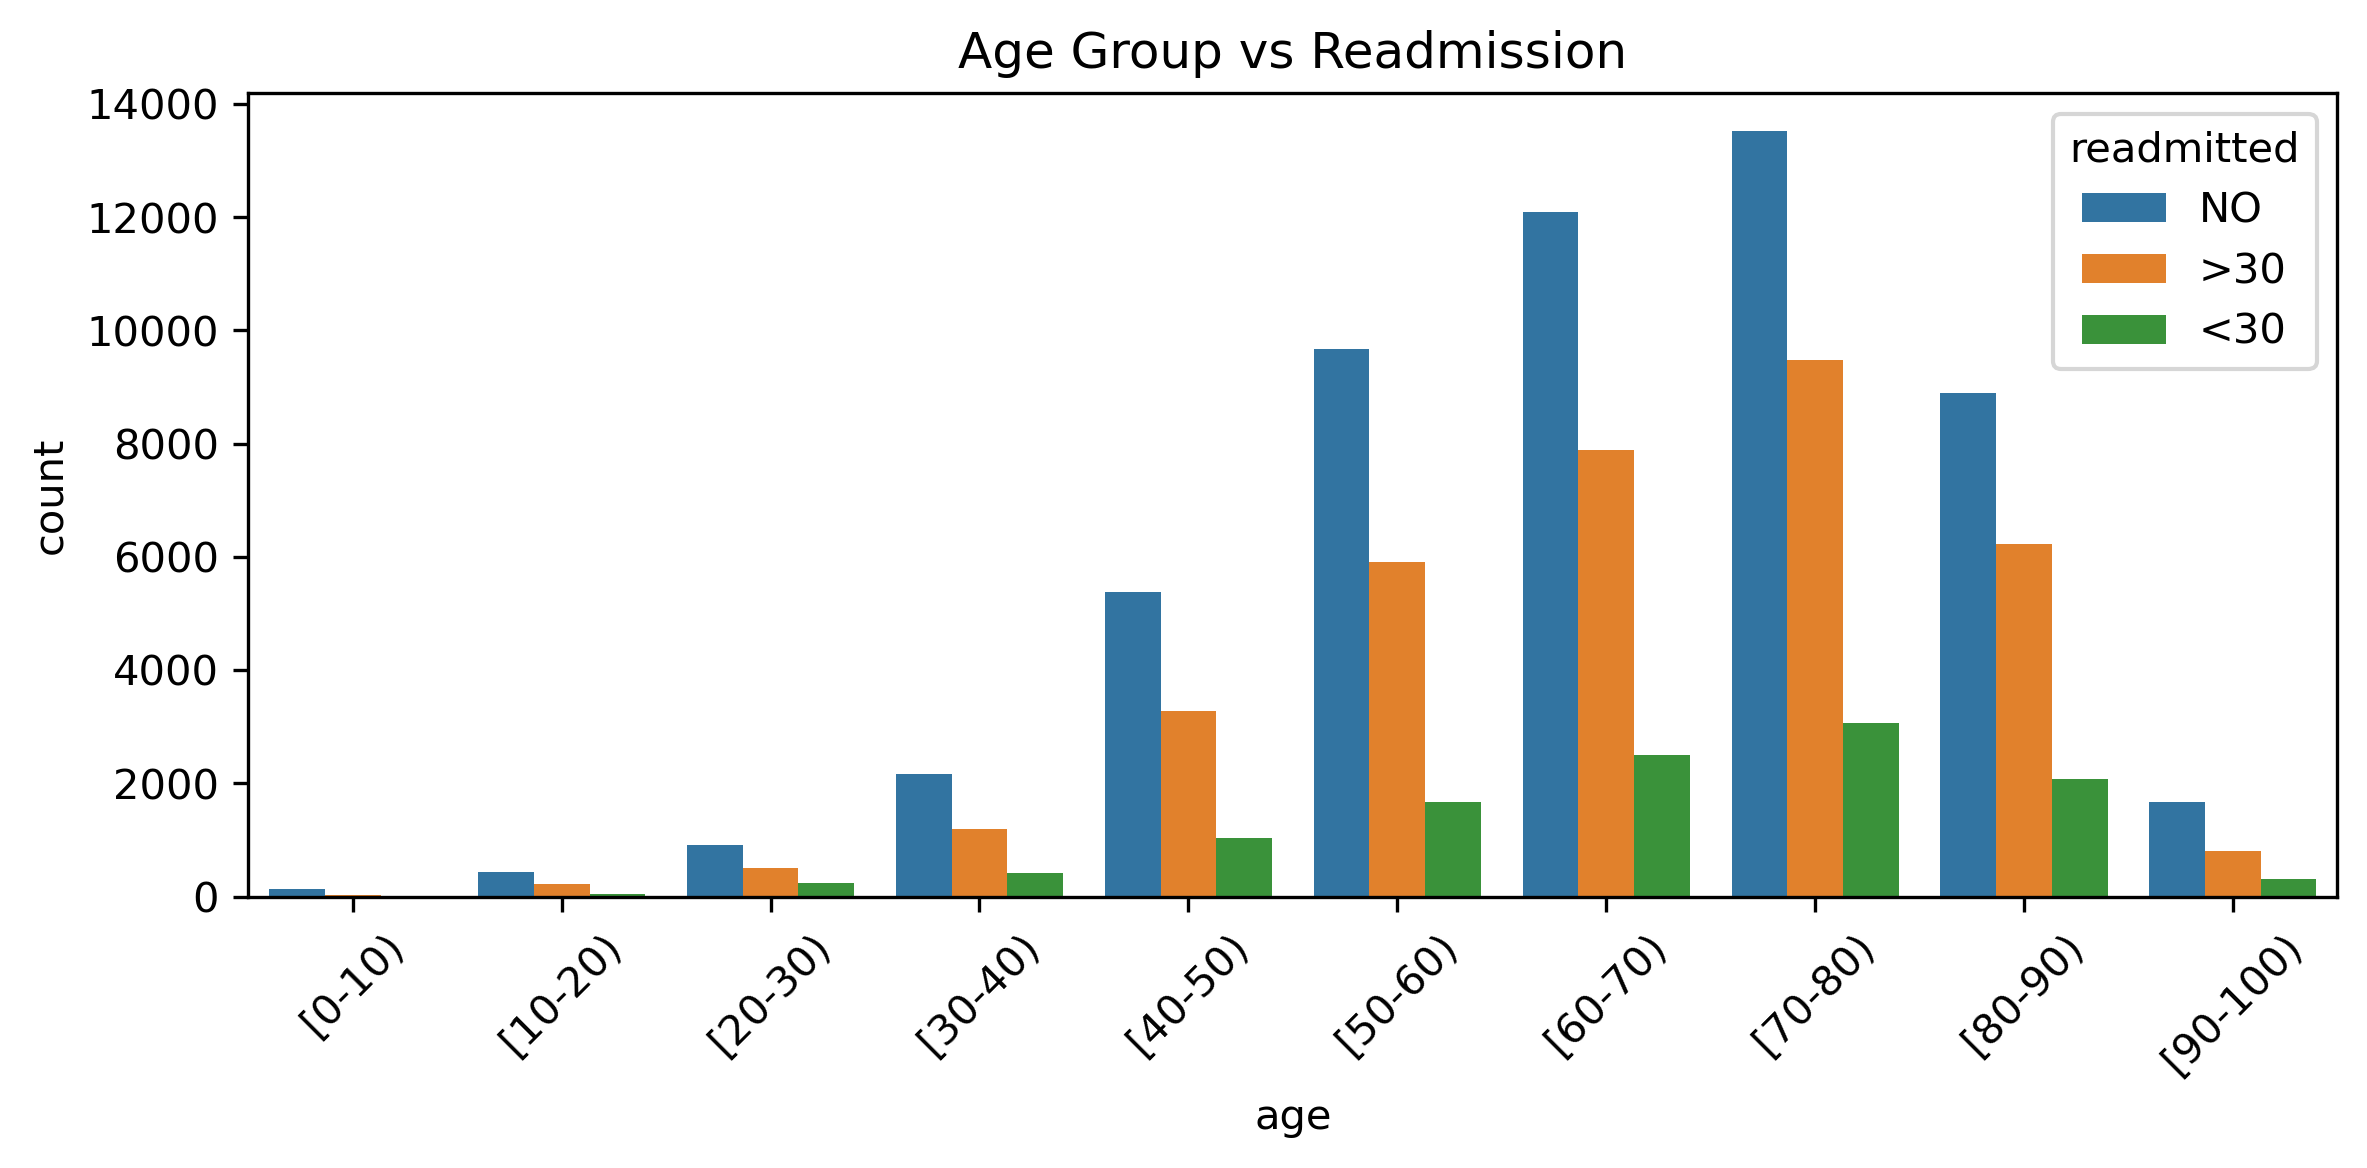
\includegraphics[width=\linewidth]{fig_age_vs_readmit.png}
\caption{Age group vs.\ readmission, suggests higher risk in older patients.}
\end{minipage}
\label{fig:eda1}
\end{figure}

\subsection{Missingness and feature design}

Several variables use \texttt{?} as a missing-value code.
Figure 3 shows that \texttt{weight}, \texttt{payer\_code}, \texttt{max\_glu\_serum}, \texttt{medical\_specialty}, and \texttt{medical\_specialty} are missing in 40--98\% of encounters.
These columns were dropped because their high missingness made them difficult to model reliably.
Diagnosis columns and key utilization variables had much lower missingness and were retained.

ICD-9 diagnosis codes were extremely high-dimensional and sparse, so we mapped the three diagnosis fields into 8 broad groups (circulatory, respiratory, digestive, endocrine/diabetes, injury, musculoskeletal, genitourinary, neoplasms, and other) using simple ranges on the numeric codes.
This grouping reduces dimensionality while keeping the same broad clinical patterns.

There were 21 diabetes related medications with four levels (``No'', ``Steady'', ``Up'', ``Down'').
We condensed these into binary indicators for ``any use or adjustment'' versus ``no use''.
This decision was based on the observation that any non-zero level roughly indicates active management.

Hospital admission and discharge codes were grouped into a smaller set of clinically similar categories and then one-hot encoded.
Gender, diabetes medication flag (\texttt{diabetesMed}), and medication change (\texttt{change}) were coded as 0/1.
Age bands were mapped to integer codes 0--9 as seen in Figure 2. The final feature matrix contained 60 columns. 

\begin{figure}[H]
\centering
\begin{minipage}{0.47\linewidth}
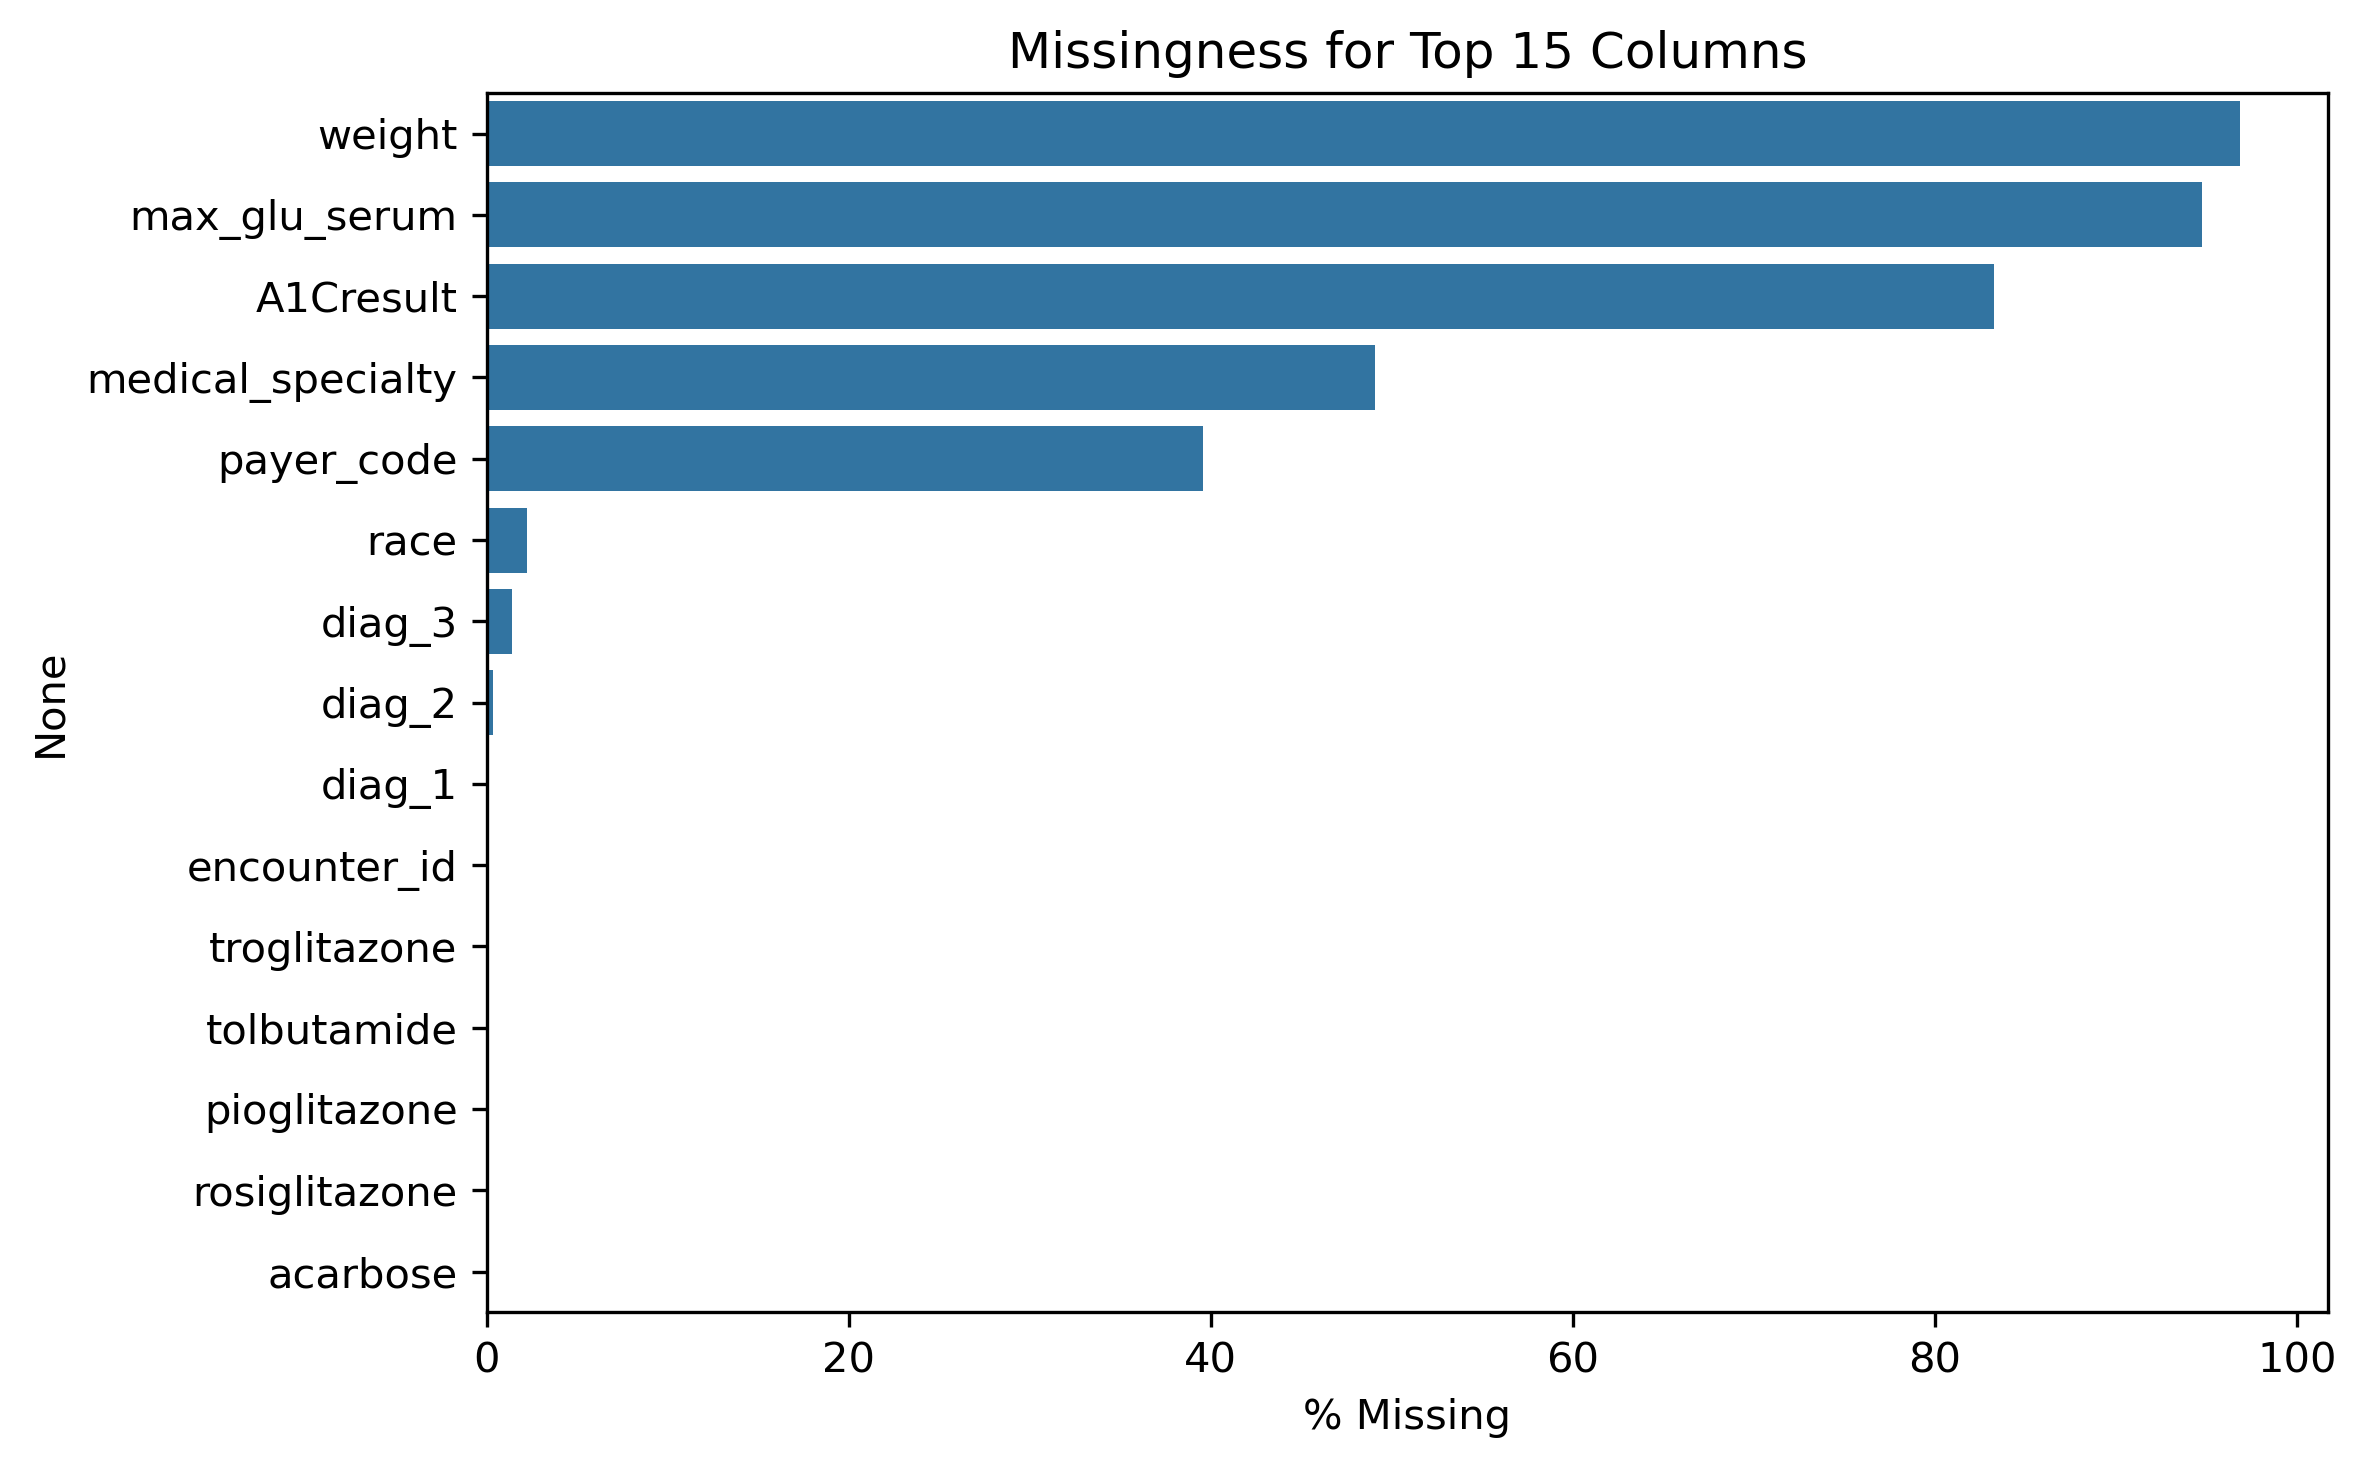
\includegraphics[width=\linewidth]{fig_missingness.png}
\caption{Missingness in the 15 most affected columns.}
\end{minipage}
\hfill
\begin{minipage}{0.47\linewidth}
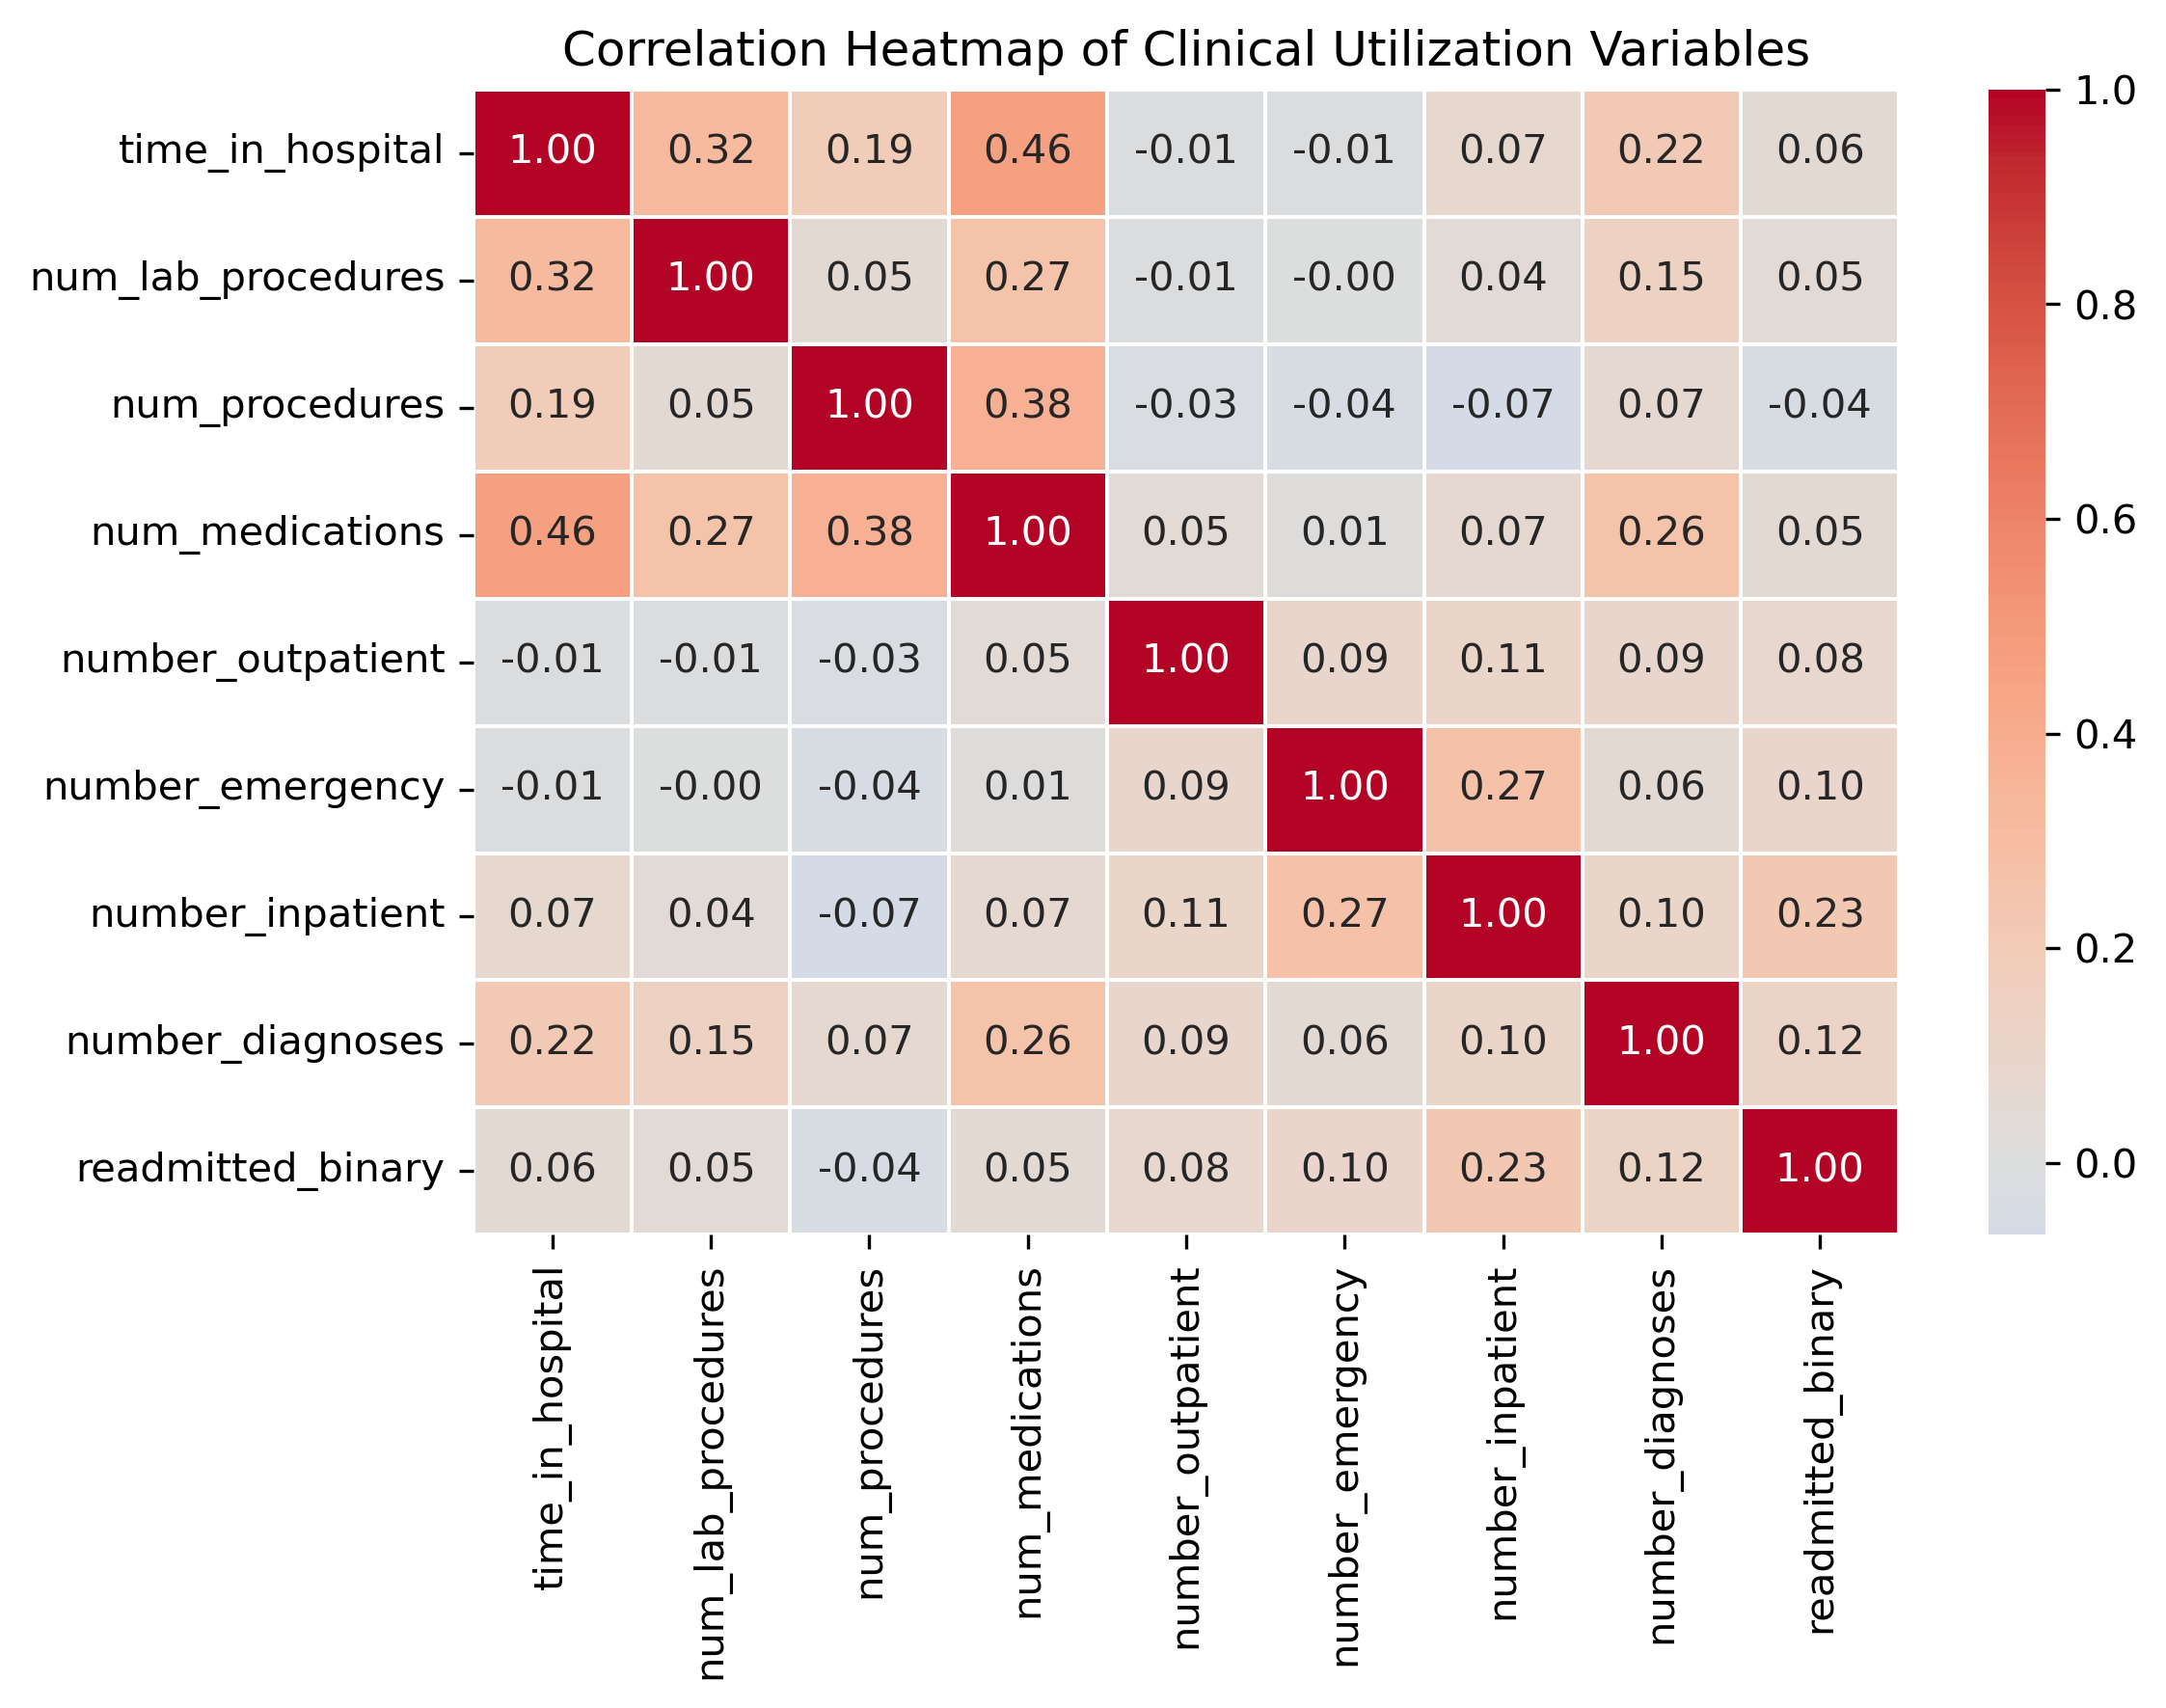
\includegraphics[width=\linewidth]{fig_correlation.png}
\caption{Correlation matrix of key numeric clinical variables.}
\end{minipage}
\end{figure}

\subsection{Train--test split and balancing}

We used an 80/20 stratified split to make our training and testing sets.
To improve model training, we addressed class imbalance only in the training set. The not readmitted class was downsampled to match the readmitted class, to produce a balanced training sample of 37{,}453 readmitted and 37{,}453 non-readmitted encounters.
The test set retained the original 53/47 prevalence so that evaluation reflects the real clinical distribution.

A \texttt{StandardScaler} was fit on the balanced training features and then applied to both training and test sets for models that change based on feature scaling (Logistic Regression, SVM, and MLP).
Tree-based models (Decision Trees and Random Forests) used the unscaled features.

\section{Models and Hyperparameter Selection}

We implemented four models:
Logistic Regression, Random Forests, SVMs with RBF kernel, and MLP Neural Networks.
Our emphasis was on how we chose hyperparameters and controlled complexity.
Stratified k--fold cross-validation on the balanced training data was used throughout for model comparison and tuning, with ROC--AUC as the primary score.

\subsection{Logistic Regression}

Logistic Regression serves as a baseline and a check for the more complex models.
We used solver = \texttt{lbfgs}, class weights = \texttt{balanced}, and maximum iterations= 300
This configuration requires less tuning and provides interpretable coefficients.
It also gives a point of comparison for how much benefit the nonlinear models provide.

\subsection{Random Forests}

\begin{figure}[H]
\centering
\begin{minipage}{0.47\linewidth}
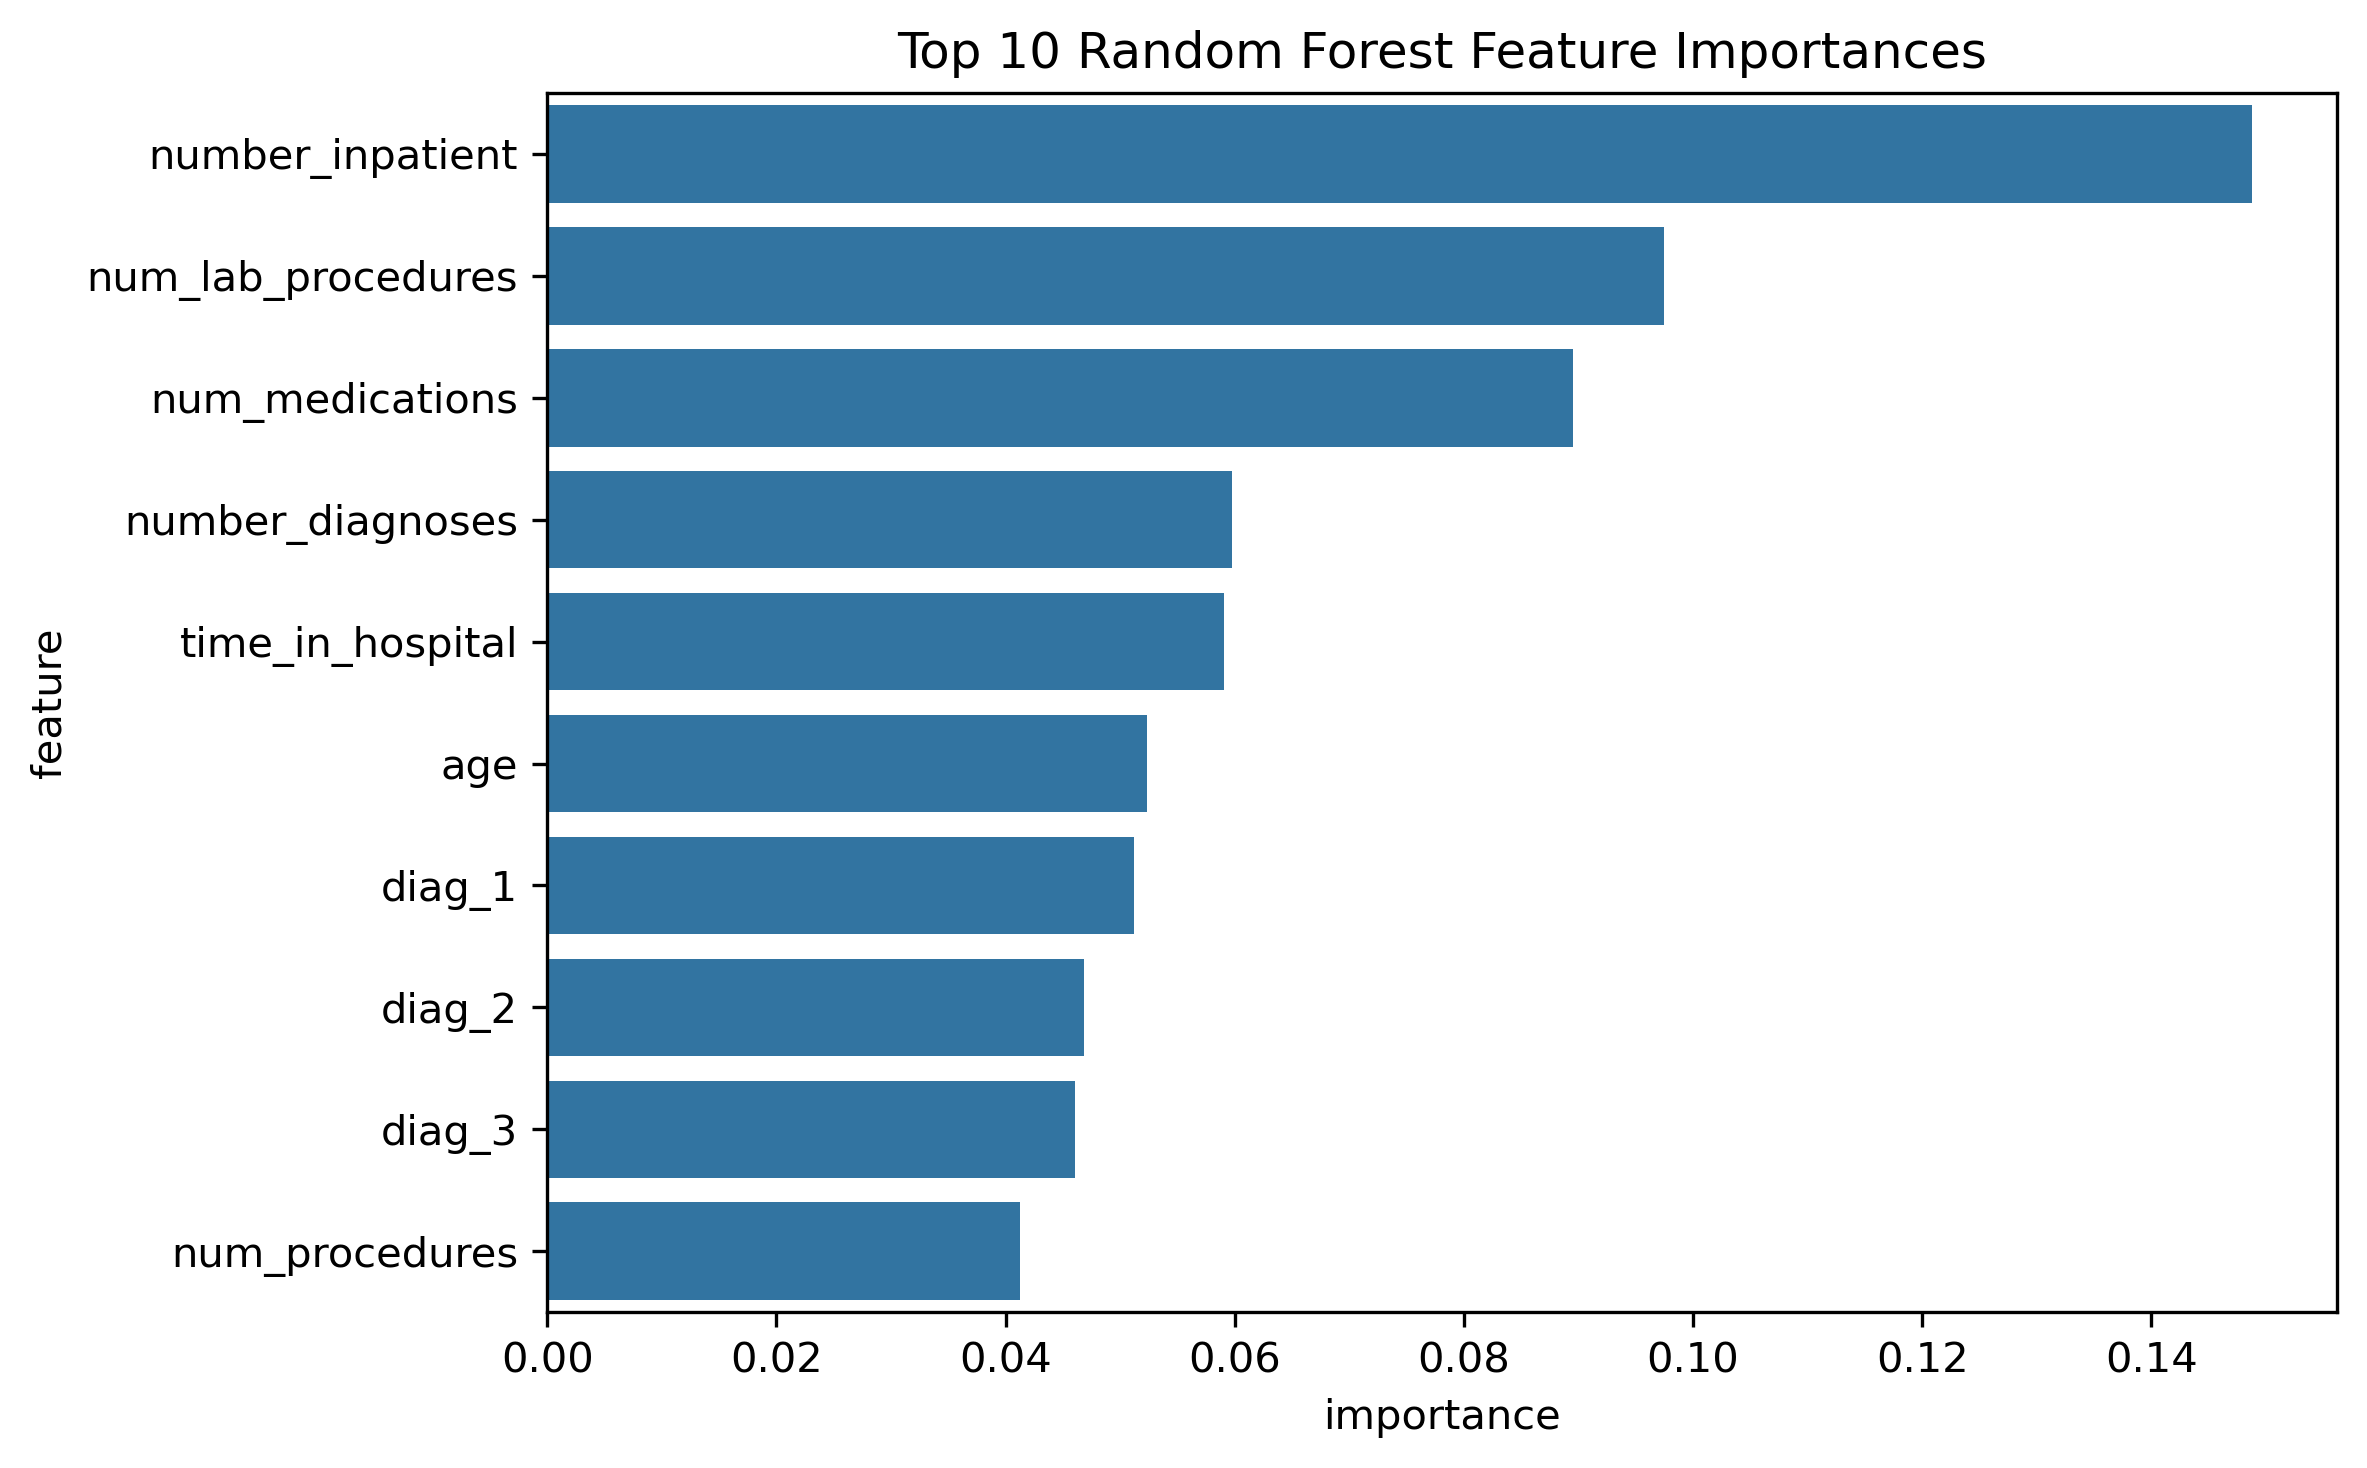
\includegraphics[width=\linewidth]{fig_rf_feature_importance.png}
\caption{Top Random Forest features. Prior inpatient use most important.}
\end{minipage}
\hfill
\begin{minipage}{0.47\linewidth}
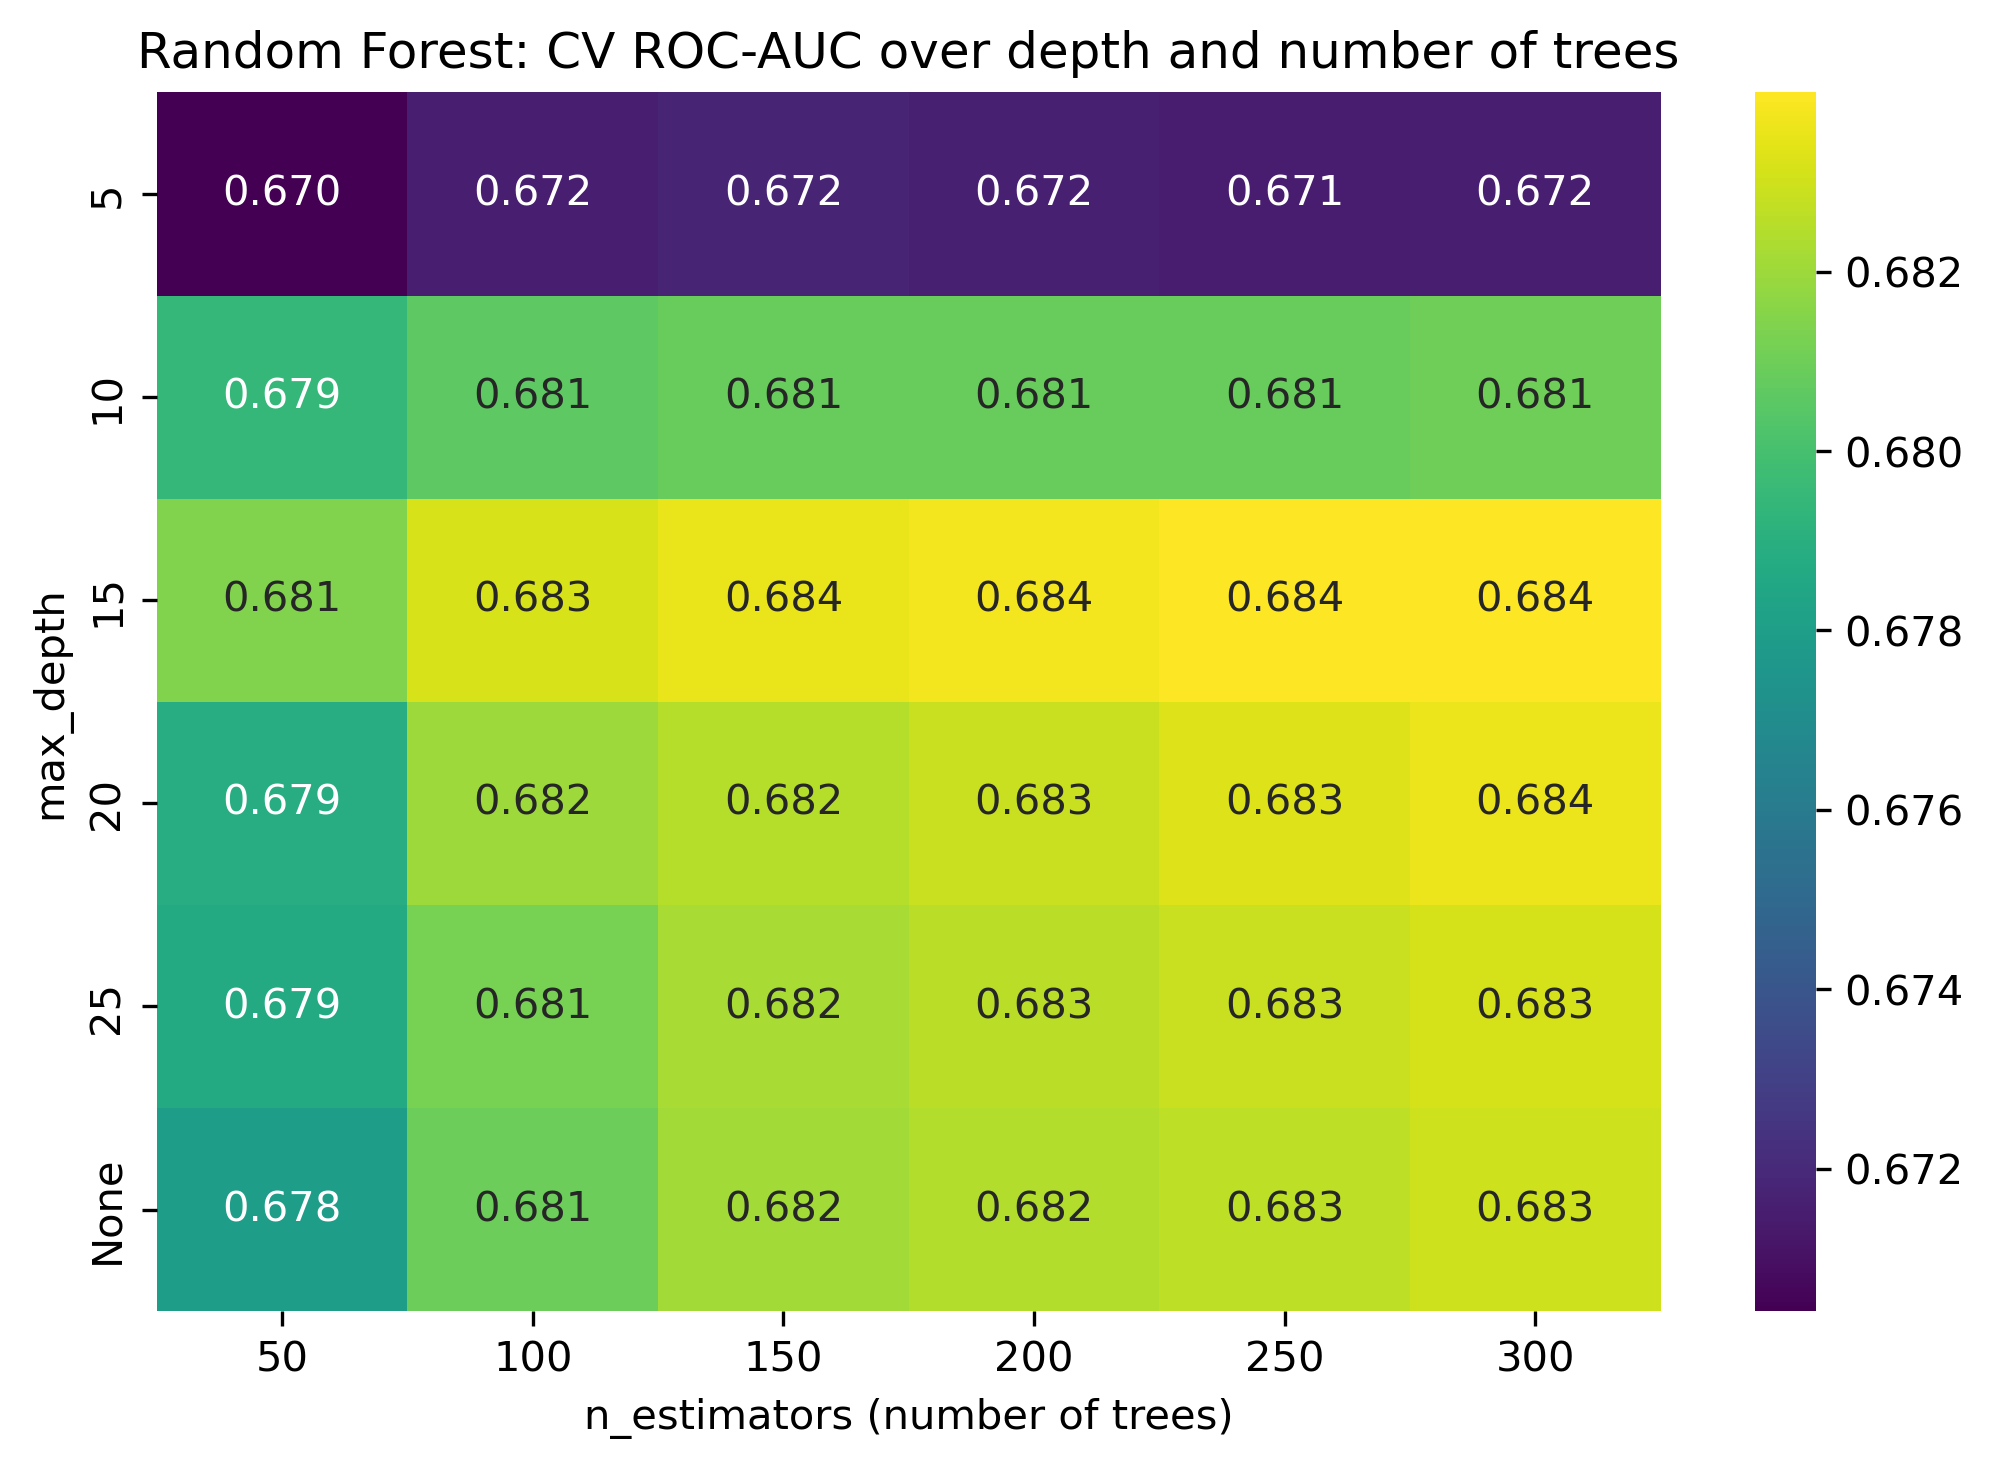
\includegraphics[width=\linewidth]{fig_rf_depth_vs_estimators.png}
\caption{Random Forest CV ROC--AUC over a grid of \texttt{max\_depth} and \texttt{n\_estimators}.}
\end{minipage}
\end{figure}



The feature importance profile ranked number of inpatient visits, number of lab procedures, and number of medications
as the strongest predictors of readmission which makes sense logically.
To evaluate model sensitivity, we also varied both \texttt{max\_depth} and 
\texttt{n\_estimators} and observed that models deeper than 20 began to overfit, while 
increasing the number of trees beyond 200 yielded diminishing returns.

Random Forests are a good choice for this dataset because the dataset deals with a mix of continuous and categorical variables.
They also capture interactions between features such as diagnoses, prior utilization, and medication use and are relatively robust to noise and outliers.

We manually explored a set of parameter combinations based on bias--variance considerations \texttt{n\_estimators}, \texttt{max\_depth}, and \texttt{min\_samples\_leaf}.

For each configuration we computed 5-fold stratified CV ROC--AUC.

Depth values larger than 20 gave training accuracy close to 1.0 but did not improve validation AUC, indicating overfitting.
Increasing \texttt{min\_samples\_leaf} from 1 to 5 slightly reduced training performance but improved validation performance and stabilized feature importance.

The best model (tuned Random Forest) according to cross-validation with mean CV ROC--AUC $\approx 0.685$ was \texttt{n\_estimators} = 200, \texttt{max\_depth} = 20, \texttt{min\_samples\_leaf} = 5.



\subsection{Support Vector Machine (RBF)}

We looked at SVMs with RBF kernel as a nonlinear model.
However, training RBF SVMs on tens of thousands of samples is computationally expensive ($\mathcal{O}(n^2)$).
To keep training feasible we subsampled 20{,}000 examples from the balanced training set, used \texttt{C = 1.0} as a moderate regularization strength, used \texttt{gamma = scale}, which adapts the kernel width to the feature dimensionality, and set \texttt{class\_weight = balanced}.

Under these settings, SVM performance on the test set was comparable to Logistic Regression but did not surpass the tuned Random Forest or MLP with a CV ROC--AUC $\approx 0.664$ at gamma = 0.001 and C = 10.

\subsection{Multilayer Perceptron (MLP)}

\begin{figure}[H]
\centering
\begin{minipage}{0.47\linewidth}
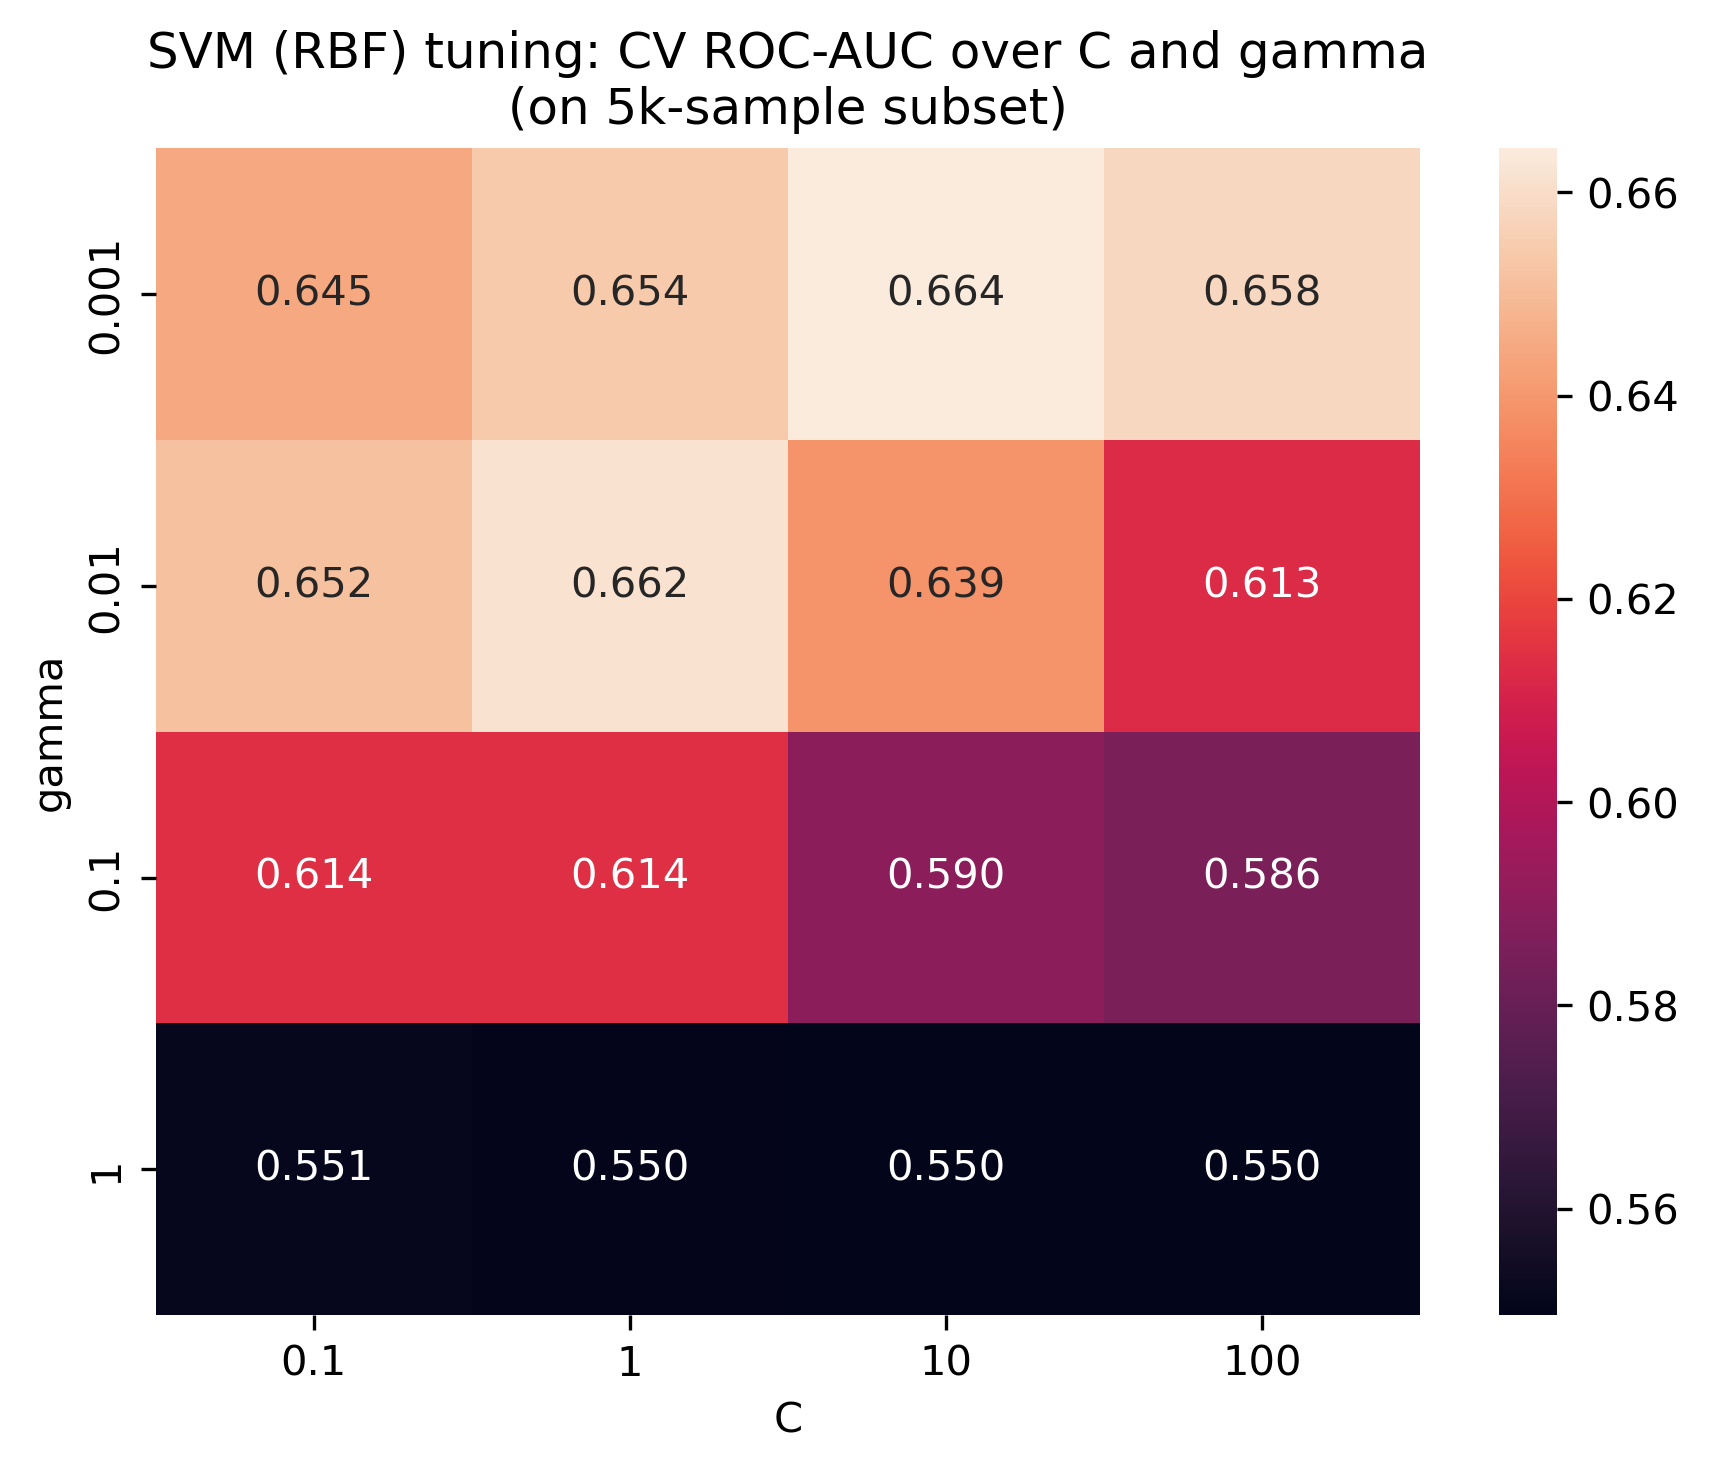
\includegraphics[width=\linewidth]{fig_svm_tuning_heatmap.png}
\caption{SVM (RBF) tuning: $C$ and $\gamma$.}
\end{minipage}
\hfill
\begin{minipage}{0.47\linewidth}
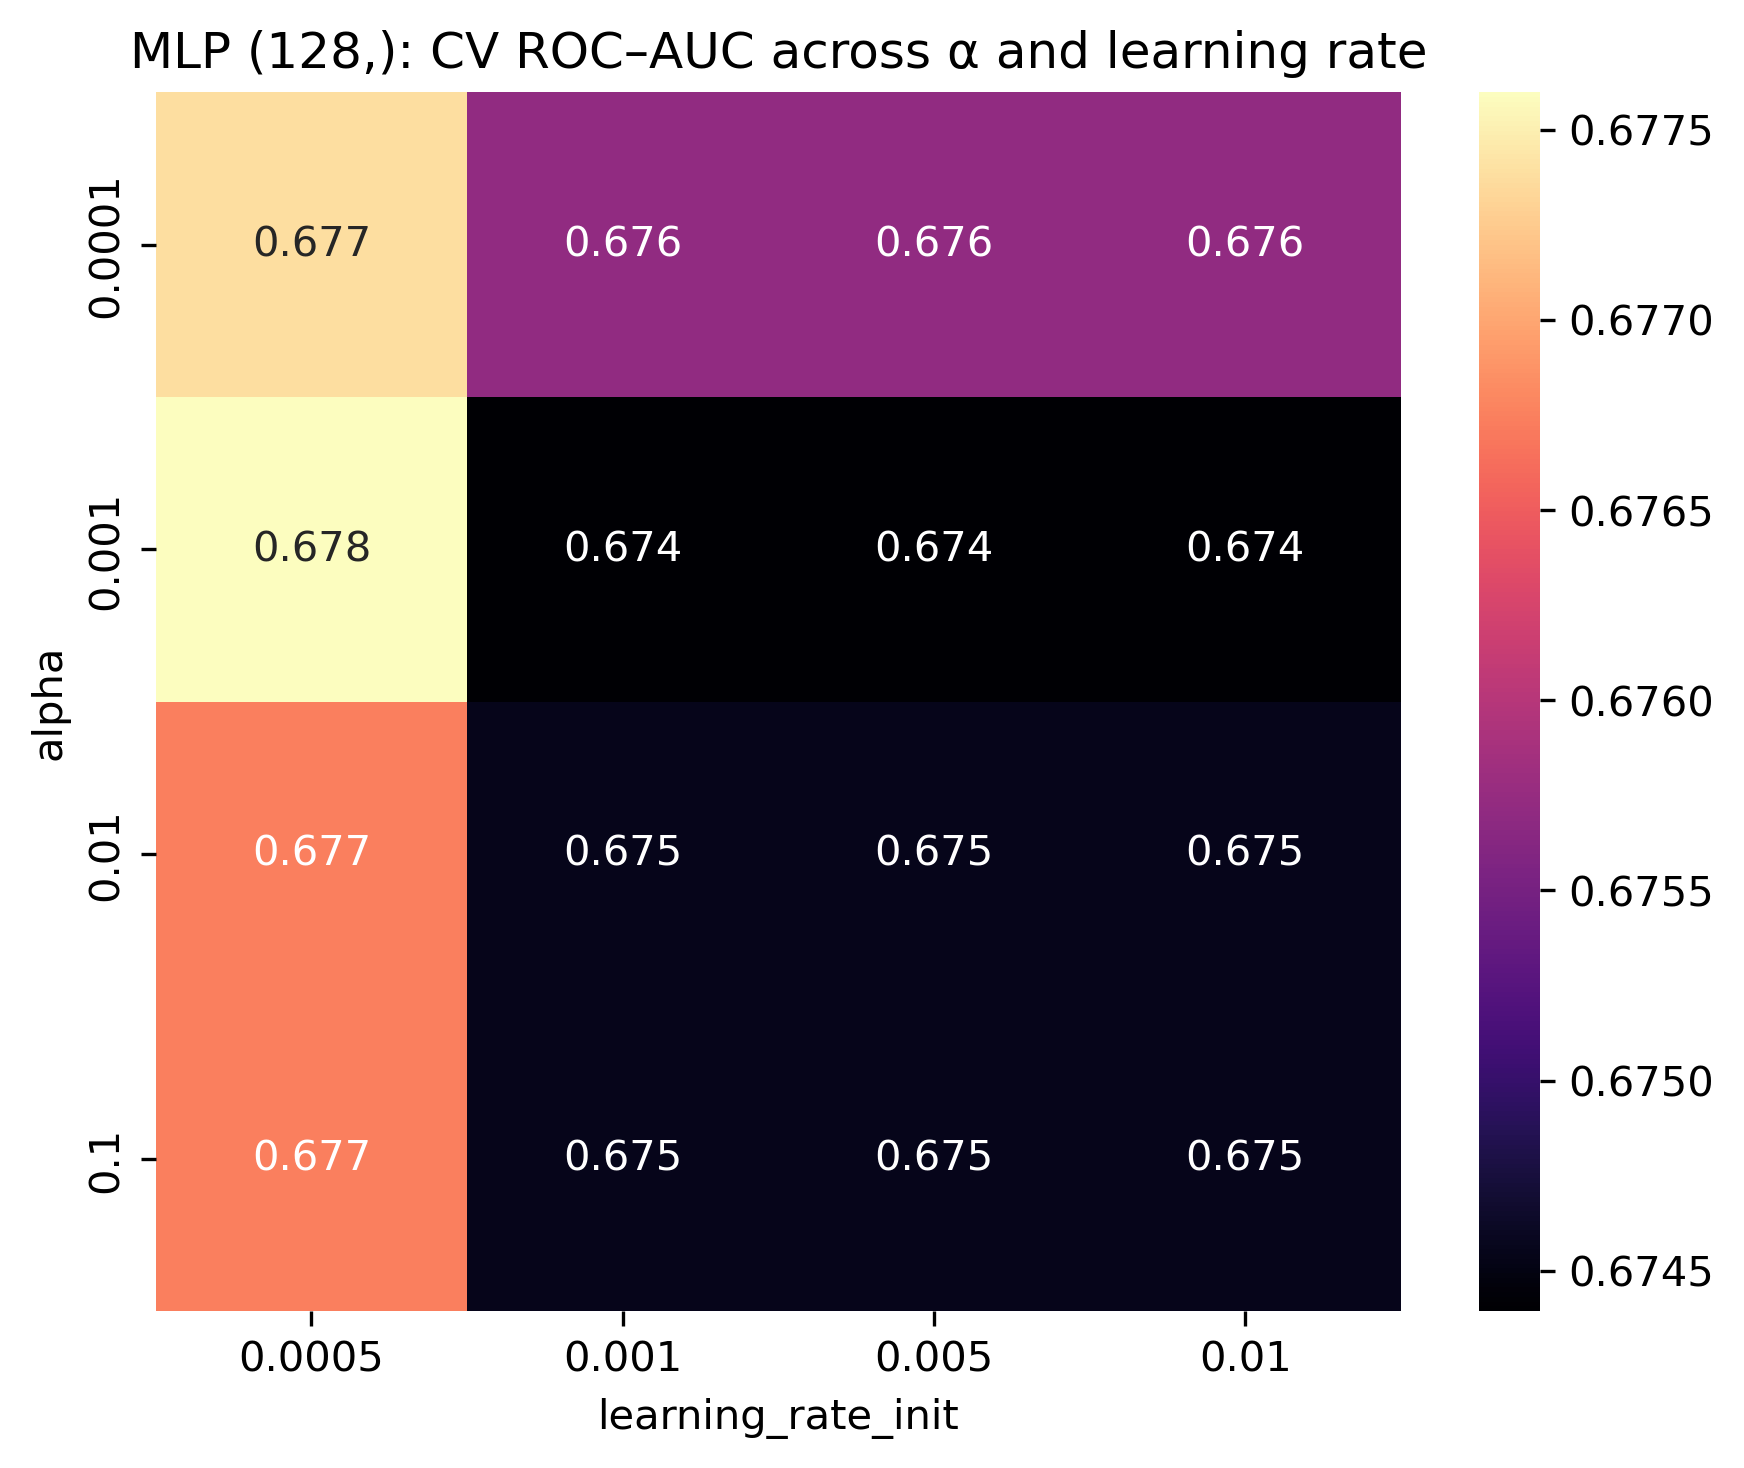
\includegraphics[width=\linewidth]{fig_mlp_hyperparam_heatmap.png}
\caption{MLP tuning: $\alpha$ and learning rate.}
\end{minipage}
\end{figure}



The MLP is the most flexible model considered here and required careful complexity control.
The dataset has only moderate signal-to-noise ratio and relatively simple structure, so very deep networks risk severe overfitting.

We varied three aspects of the architecture and optimization which included hidden layer structures, L2 regularization strength, and initial learning rate.

Other settings were fixed such as ReLU activations, batch size 256, maximum 50 epochs, and early stopping based on validation loss.

Figure 10 shows a complexity curve where we vary only the hidden layer size and plot mean training and validation accuracy across CV folds.
Training accuracy steadily increases with network size, while validation accuracy is nearly flat and drops for the $(128, 64)$ architecture, indicating some overfitting.

The chosen configuration (tuned MLP) balances model flexibility with generalization with a CV ROC--AUC $\approx 0.678$, a single hidden layer with 128 units, $\alpha=0.001$, and learning rate $5\times 10^{-4}$.

\section{Validation, Complexity, and Results}

\subsection{Under-fitting and Over-fitting}

To visualize under-fitting and over-fitting explicitly, we examined decision trees with different maximum depths and MLPs with different hidden sizes.

\begin{figure}[H]
\centering
\begin{minipage}{0.47\linewidth}
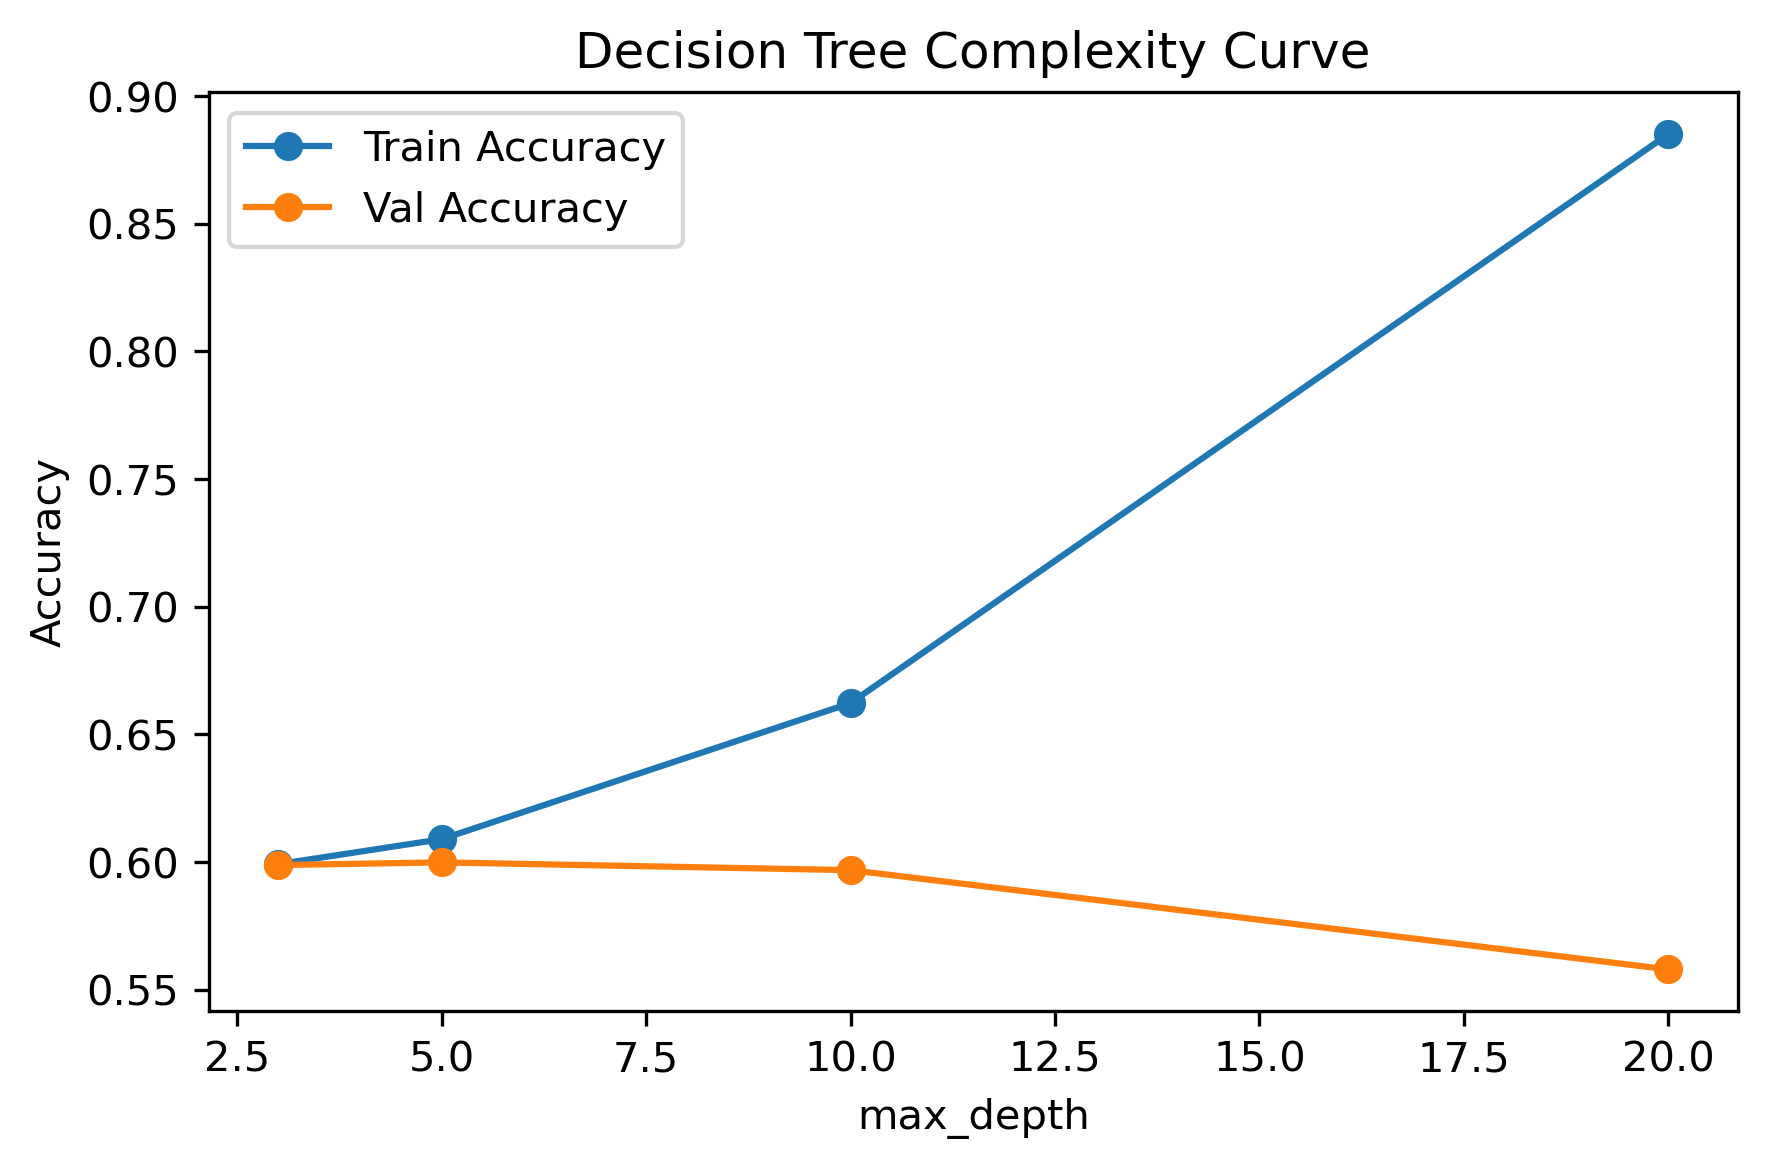
\includegraphics[width=\linewidth]{fig_complexity_curve.png}
\caption{Decision tree complexity curve: deep trees overfit.}
\end{minipage}
\hfill
\begin{minipage}{0.47\linewidth}
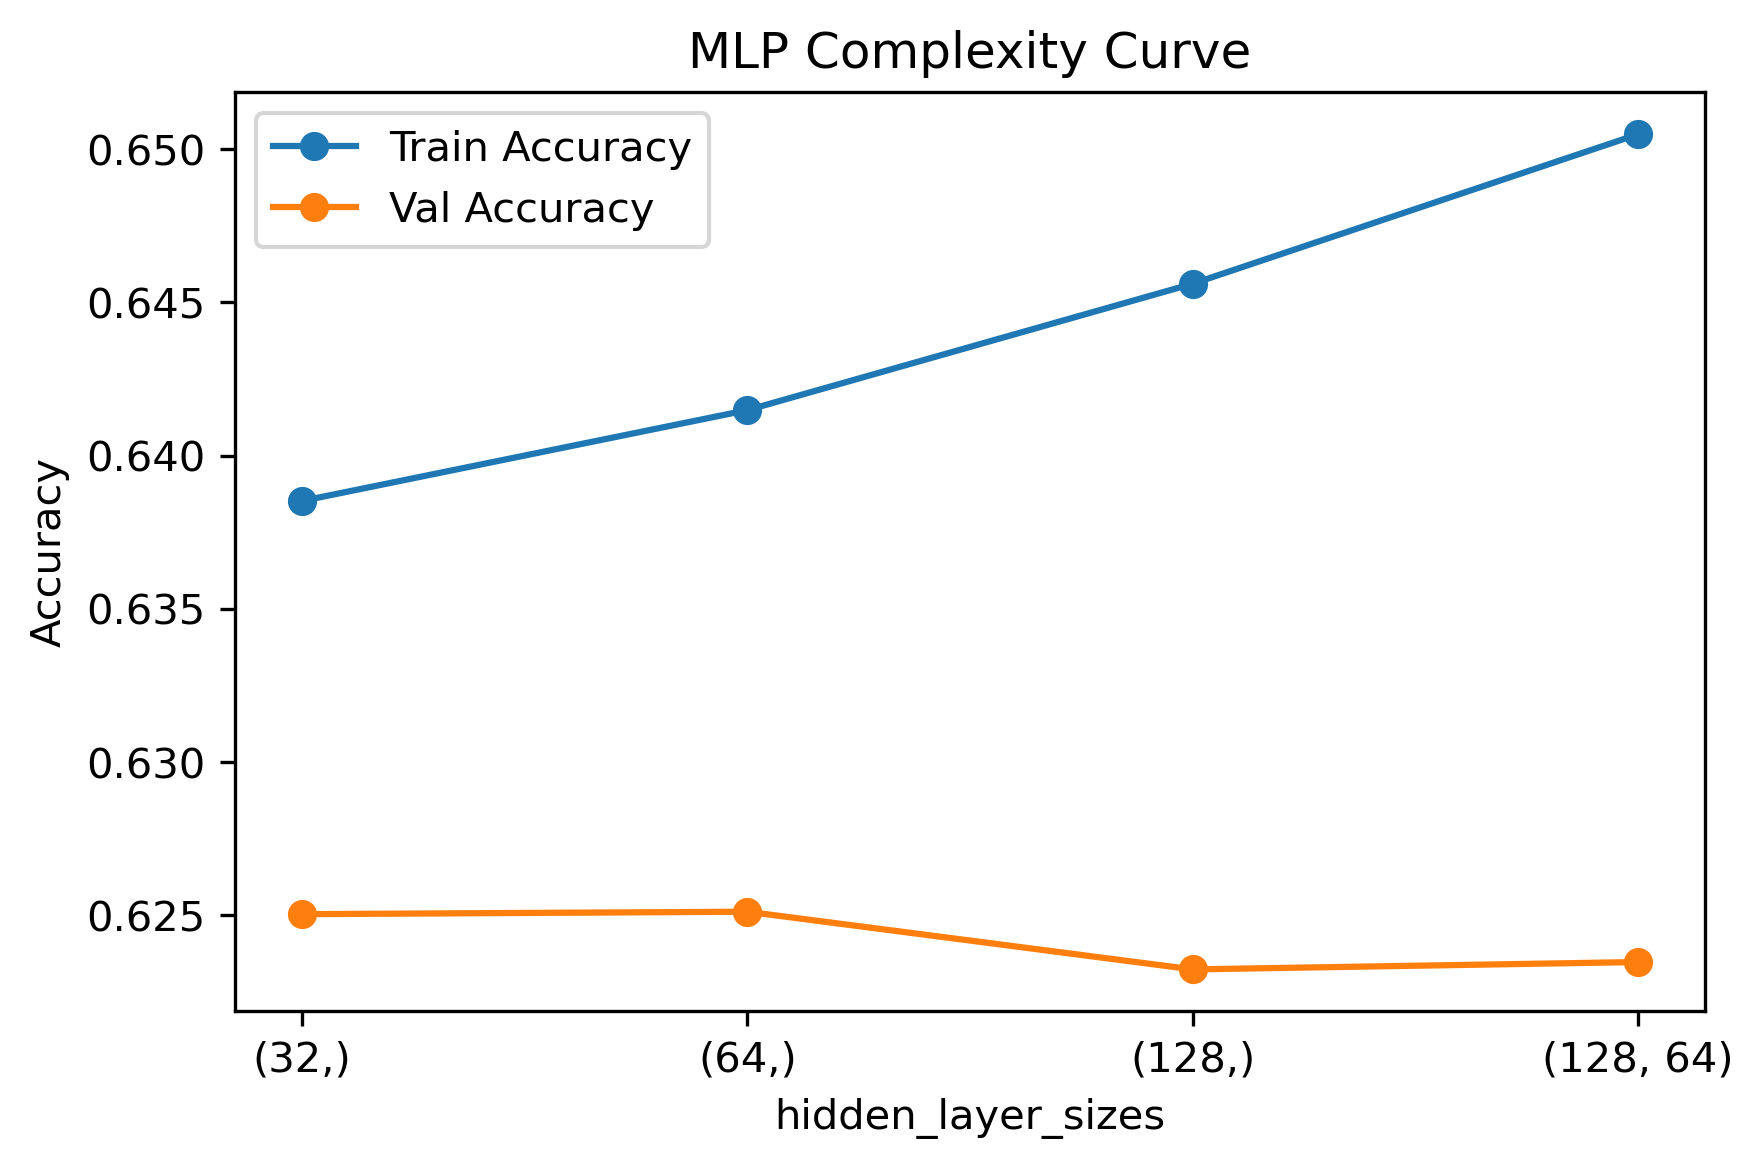
\includegraphics[width=\linewidth]{fig_mlp_complexity.png}
\caption{MLP complexity curve: larger networks give small gains before overfitting.}
\end{minipage}
\label{fig:complex}
\end{figure}

For trees, validation accuracy peaked at depth around 5--10 and decreased after, which is the expected behavior of high variance.
This motivated using Random Forests with moderate depth and a nontrivial \texttt{min\_samples\_leaf}.
For the MLP, the gap between training and validation accuracy remained small, but the $(128, 64)$ network began to lose validation performance, suggesting that a single hidden layer is sufficient.

\subsection{Test-set performance}

All models were trained on the balanced training set (with scaling where appropriate) and evaluated on the original test set of 19{,}868 encounters.
Table 1 summarizes performance. Figure 11 provides a visual comparison of the same metrics and Figure 12 shows ROC curves.


The tuned Random Forest achieves the best overall score (ROC--AUC $\approx 0.69$) and a slightly higher F1 score than the other models.
The tuned MLP attains the highest recall, which may be desirable when making sure not to miss high-risk patients is important.
Logistic Regression and SVM perform similarly, indicating that while the relationship between predictors and readmission is somewhat nonlinear, the benefit of complex kernels is limited by noise and feature quality.
All models perform better than just guessing, but the curves illustrate only slight separation between the models.

\begin{table}[H]
\centering
\begin{tabular}{lccccc}
\toprule
Model & Accuracy & Precision & Recall & F1 & ROC--AUC \\
\midrule
Logistic Regression (balanced) & 0.63 & 0.62 & 0.55 & 0.58 & 0.67 \\
Random Forest (fixed)          & 0.64 & 0.62 & 0.60 & 0.61 & 0.69 \\
MLP (fixed 128--64)            & 0.63 & 0.61 & 0.60 & 0.60 & 0.68 \\
SVM (RBF)                      & 0.62 & 0.60 & 0.60 & 0.60 & 0.67 \\
Random Forest (tuned)          & \textbf{0.64} & \textbf{0.62} & 0.61 & \textbf{0.62} & \textbf{0.69} \\
MLP (tuned 128)                & 0.63 & 0.60 & \textbf{0.63} & 0.61 & 0.68 \\
\bottomrule
\end{tabular}
\caption{Test performance. Values are rounded to two decimals.}
\label{tab:results}
\end{table}

\begin{figure}[H]
\centering
\begin{minipage}{0.47\linewidth}
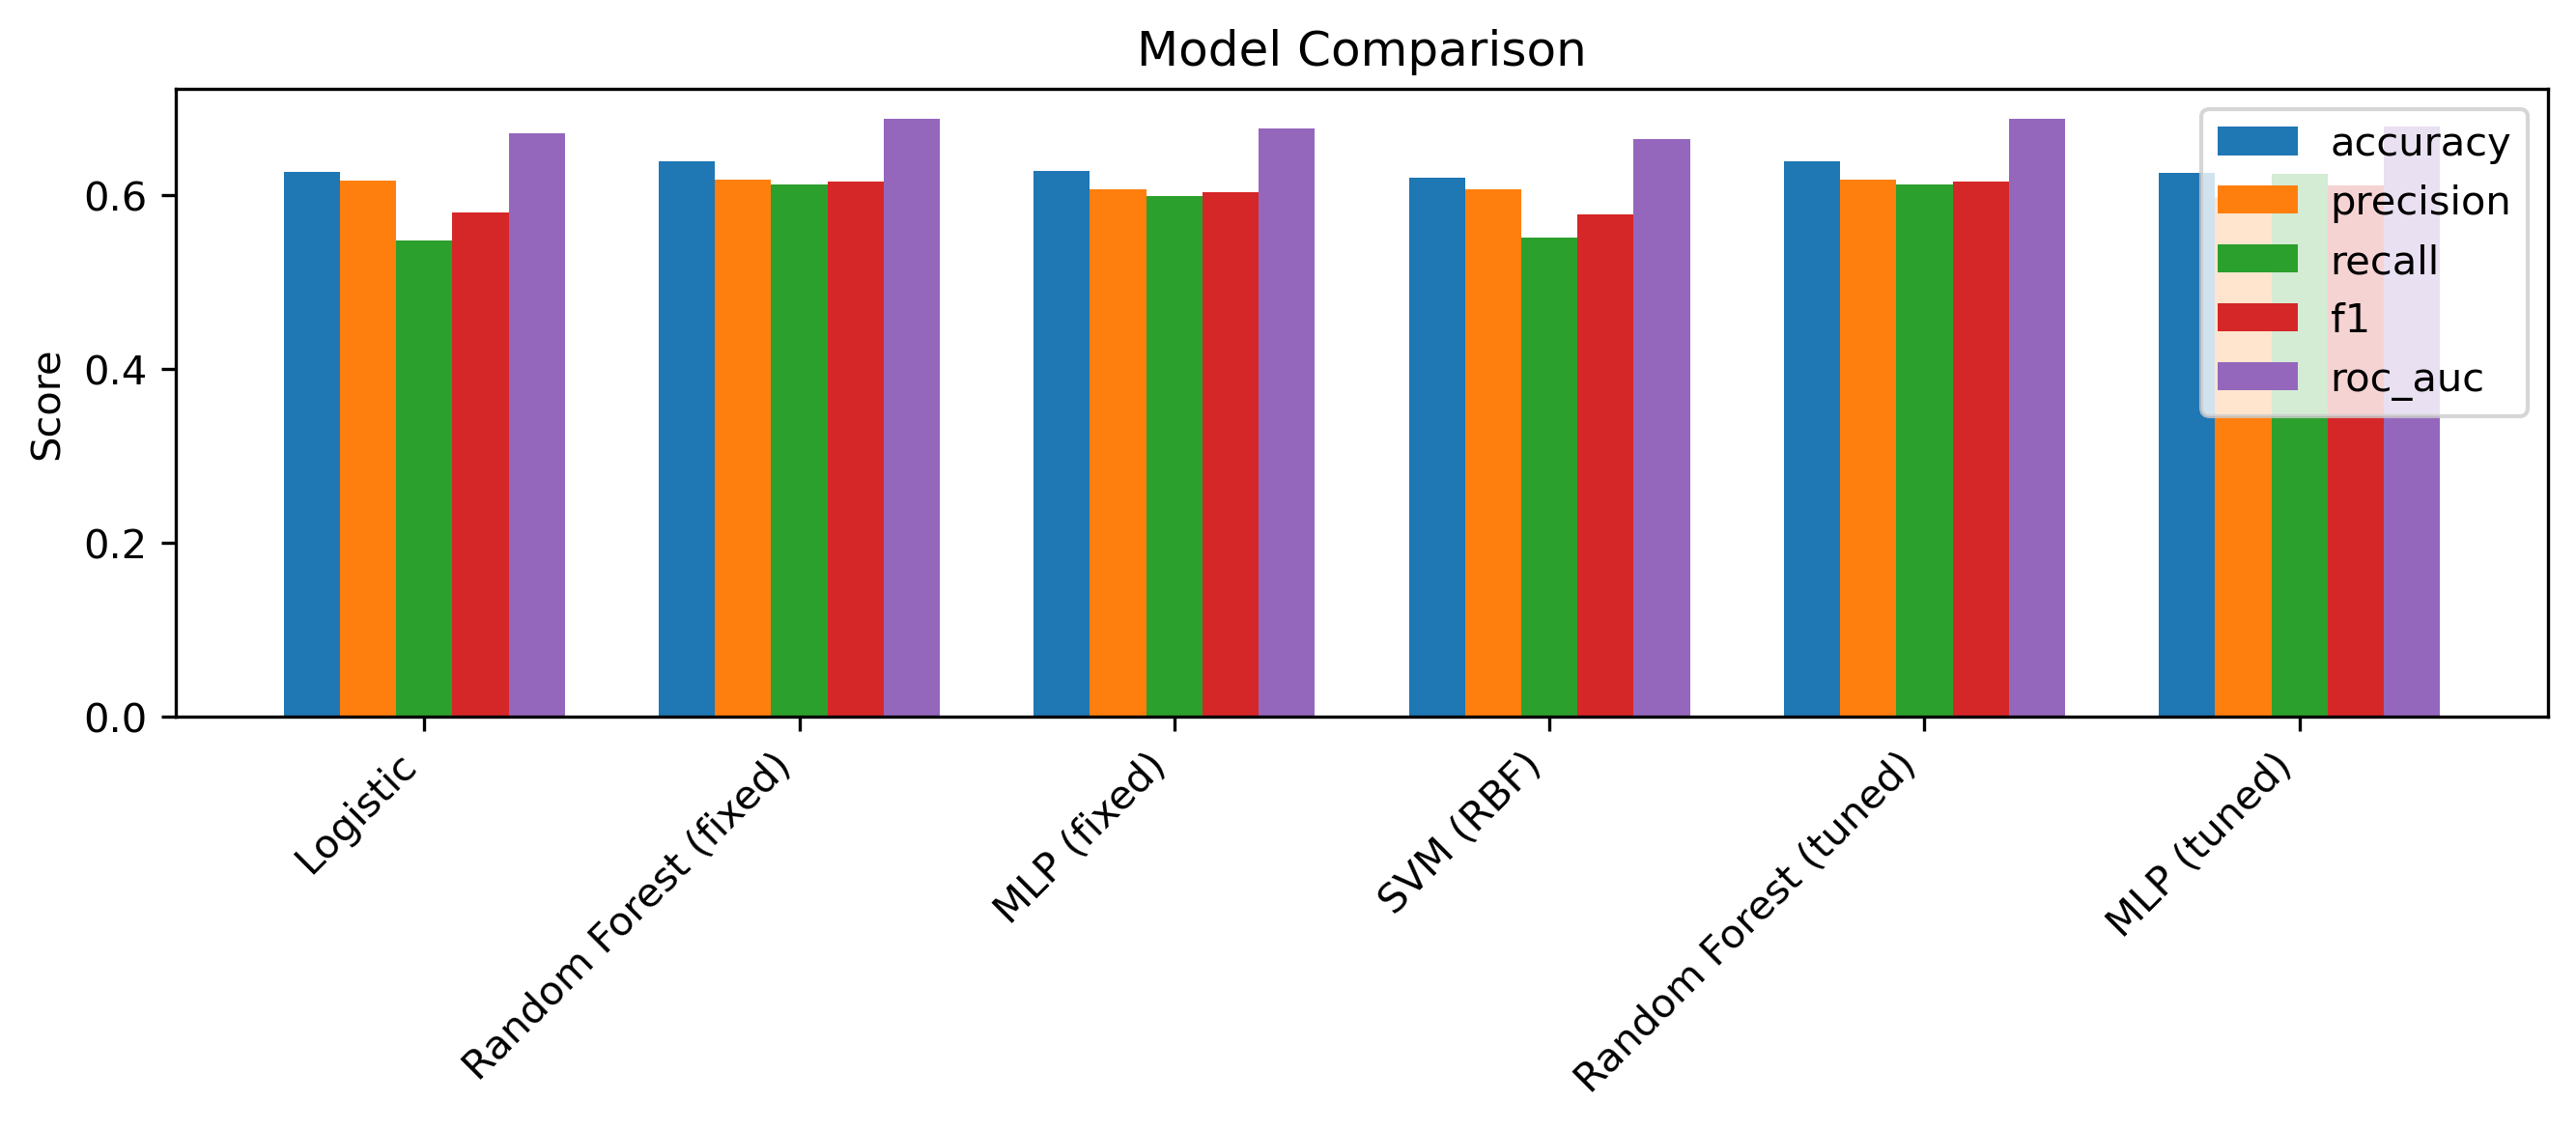
\includegraphics[width=\linewidth]{fig_model_comparison.png}
\caption{Comparison of accuracy, precision, recall, F1, and ROC--AUC for all models.}
\end{minipage}
\hfill
\begin{minipage}{0.47\linewidth}
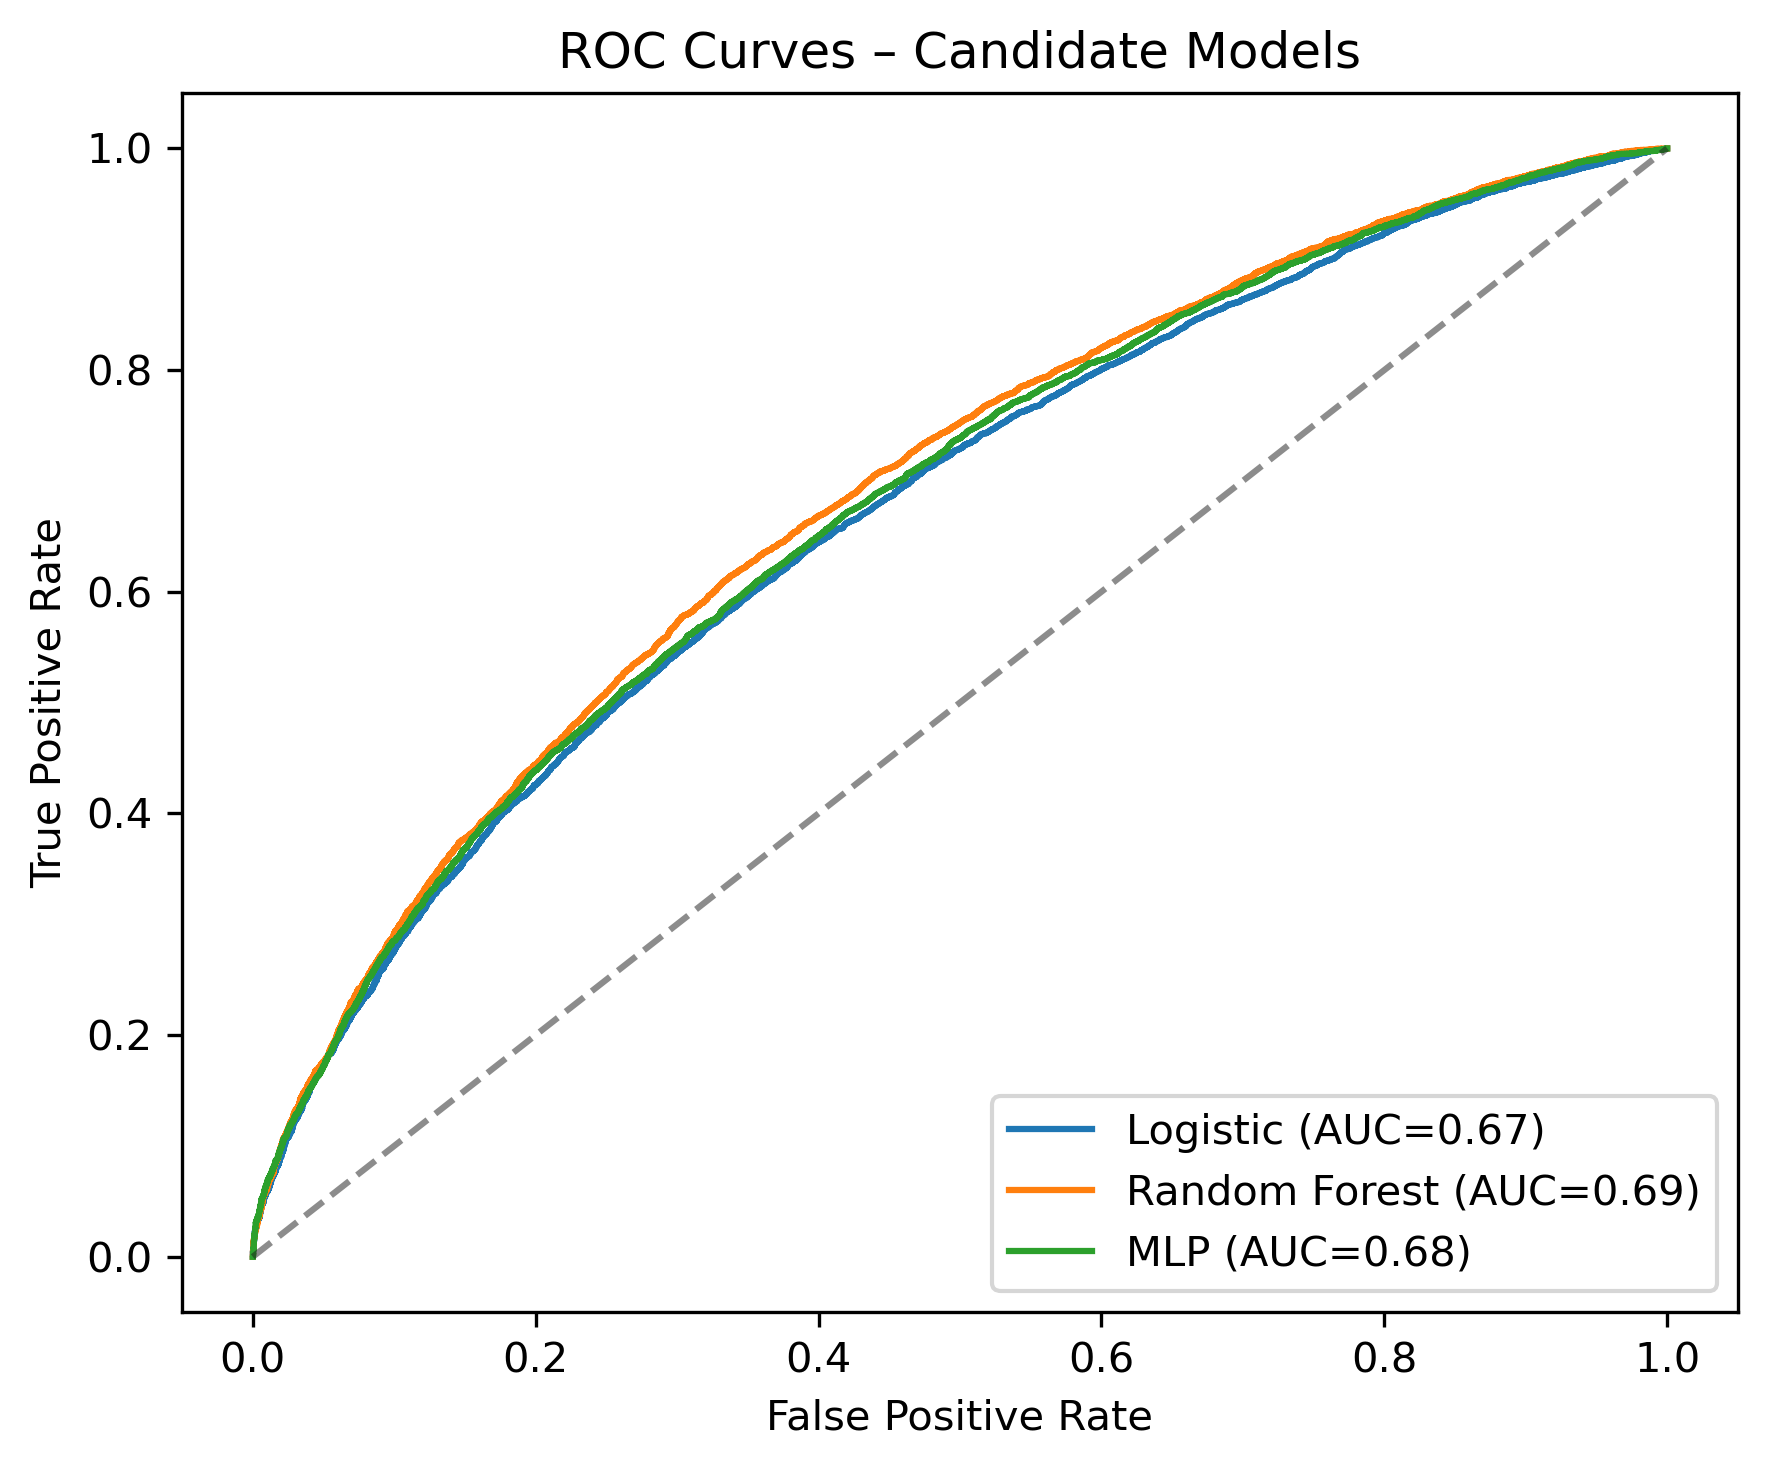
\includegraphics[width=\linewidth]{fig_roc_curves.png}
\caption{ROC curves for Logistic Regression, tuned Random Forest, and tuned MLP.}
\end{minipage}
\end{figure}


\section{Discussion and Conclusion}

This project illustrates a full machine learning workflow on a real clinical dataset, with a focus on how model and parameter choices are influenced by the data and effect results.

Exploratory analysis revealed heavy missingness in some variables and highlighted the importance of healthcare utilization measures and diagnosis groups.
Feature engineering focused on grouping ICD-9 codes, making medication use binary, and encoding hospital identifiers.
Balancing the training set by downsampling the majority class, while leaving the test set unchanged, produced models with similar precision and recall for the positive class.

Random Forests and MLPs offered the best performance, with Random Forests slightly ahead in ROC--AUC and F1, and MLPs slightly ahead in recall.
Complexity curves showed expected under-fitting and over-fitting patterns.
Deep single trees greatly overfit, whereas moderate depth ensembles and smaller sized neural networks generalize better.
SVMs with RBF kernel performed decently but did not provide clear gains over simpler models. This could possibly due to computational constraints and noisy features.


\section*{Team Contributions}

All members contributed to interpreting results and writing the report.
Nhan focused on EDA and cleaning, Nathan worked on LR, MLP, and ROC/complexity plots, Alex worked on Random Forests, SVMs. 

\end{document}
